\documentclass[a4paper,12pt,twoside]{report}

\usepackage{scrextend}
\changefontsizes{13pt}
\usepackage[utf8]{inputenc}
\usepackage[T5]{fontenc}
\usepackage[utf8]{vietnam}
\usepackage{times}
\usepackage[top=2cm,bottom=2cm,left=3.5cm,right=2.5cm]{geometry}
\usepackage{graphicx}
\usepackage{xcolor}
\usepackage{float}
\usepackage{array}
\usepackage{booktabs}
\usepackage{multirow}
\usepackage{enumitem}
\usepackage{indentfirst}
\usepackage{setspace}
\usepackage{parskip}
\usepackage{amsmath}
\usepackage{amsfonts}
\usepackage{amssymb}
\usepackage{amsthm}
\usepackage{bm}
\usepackage{titlesec}
\usepackage{titletoc}
\usepackage{chngcntr}
\usepackage[font=small,labelfont=bf]{caption}
\usepackage{subcaption}
\usepackage{algorithm2e}
\usepackage{listings}
\usepackage{fancyhdr}
\usepackage{xurl}
\usepackage[unicode,hidelinks]{hyperref}
\usepackage[all]{hypcap}
\usepackage{placeins}
\usepackage[backend=bibtex,style=ieee]{biblatex}

\addbibresource{Danh_sach_tai_lieu_tham_khao.bib}
\lstdefinestyle{soictcode}{
  basicstyle=\ttfamily\small,
  keywordstyle=\bfseries\color{blue!60!black},
  commentstyle=\itshape\color{green!40!black},
  stringstyle=\color{red!60!black},
  numbers=left,
  numberstyle=\tiny\color{gray},
  stepnumber=1,
  numbersep=8pt,
  frame=single,
  breaklines=true,
  tabsize=2,
  showstringspaces=false,
  captionpos=b
}

\lstset{style=soictcode}

% Danh mục thuật ngữ và từ viết tắt.
% Có thể bổ sung \newacronym hoặc \newglossaryentry nếu bật gói glossaries.


\graphicspath{{Hinhve/}}
\counterwithin{figure}{chapter}
\counterwithin{table}{chapter}
\setcounter{secnumdepth}{3}
\setcounter{tocdepth}{3}

\onehalfspacing
\setlength{\parindent}{15pt}
\setlength{\parskip}{6pt}

\titleformat{\chapter}[hang]{\centering\bfseries}{CHƯƠNG \thechapter.\ }{0pt}{}
\titlespacing*{\chapter}{0pt}{-20pt}{20pt}
\titleformat{\section}[hang]{\bfseries}{\thechapter.\arabic{section}\ \ \ }{0pt}{}
\titlespacing{\section}{0pt}{\parskip}{0.5\parskip}
\titleformat{\subsection}[hang]{\bfseries}{\thechapter.\arabic{section}.\arabic{subsection}\ \ \ }{0pt}{}
\titlespacing{\subsection}{30pt}{\parskip}{0.5\parskip}
\renewcommand\thesubsubsection{\alph{subsubsection}}
\titleformat{\subsubsection}[hang]{\bfseries}{\alph{subsubsection},\ }{0pt}{}
\titlespacing{\subsubsection}{50pt}{\parskip}{0.5\parskip}

\titlecontents{chapter}
  [0.0cm]
  {\bfseries\vspace{0.3cm}}
  {{\bfseries CHƯƠNG \thecontentslabel.\ }}
  {}
  {\titlerule*[0.3pc]{.}\contentspage}
\titlecontents{section}
  [0.0cm]
  {\vspace{0.15cm}}
  {\thecontentslabel\ }
  {}
  {\titlerule*[0.3pc]{.}\contentspage}
\titlecontents{subsection}
  [1.0cm]
  {\vspace{0.1cm}}
  {\thecontentslabel\ }
  {}
  {\titlerule*[0.3pc]{.}\contentspage}

\fancypagestyle{plain}{%
  \fancyhf{}%
  \fancyfoot[RO,RE]{\thepage}%
  \renewcommand{\headrulewidth}{0pt}%
  \renewcommand{\footrulewidth}{0pt}%
}
\pagestyle{fancy}
\fancyhf{}
\fancyhead[RE,LO]{\leftmark}
\fancyfoot[RE,LO]{\thepage}

\begin{document}

\begin{titlepage}
\thispagestyle{empty}
\begin{center}
{\textbf{\large TRƯỜNG ĐẠI HỌC BÁCH KHOA HÀ NỘI}}\\[0.3cm]
{\textbf{\large VIỆN CÔNG NGHỆ THÔNG TIN VÀ TRUYỀN THÔNG}}\\[3.2cm]

{\textbf{\huge ĐỒ ÁN TỐT NGHIỆP}}\\[1.0cm]
{\textbf{\Large Nền tảng chia sẻ ảnh trực tuyến tích hợp kiểm duyệt tự động, tìm kiếm ngữ nghĩa và cơ chế thành viên cho người sáng tạo}}\\[1.2cm]

{\textbf{\large Sinh viên thực hiện: \underline{\hspace{6cm}}}}\\[0.3cm]
{\large Email: \underline{\hspace{7cm}}}\\[0.8cm]
{\textbf{\large Ngành: Công nghệ thông tin}}\\[0.2cm]
{\textbf{\large Chuyên ngành: \underline{\hspace{5cm}}}}\\[1.8cm]

\begin{table}[H]
\centering
\begin{tabular}{ll}
\textbf{Giảng viên hướng dẫn:} & \underline{\hspace{7cm}} \\[0.5cm]
\textbf{Bộ môn:} & \underline{\hspace{7cm}} \\[0.5cm]
\textbf{Viện:} & Công nghệ thông tin và Truyền thông \\[0.5cm]
\end{tabular}
\end{table}

\vfill
{\textbf{HÀ NỘI, 06/2026}}
\end{center}
\end{titlepage}

\begin{titlepage}
\thispagestyle{empty}
\begin{center}
{\textbf{\large ĐẠI HỌC BÁCH KHOA HÀ NỘI}}\\[0.3cm]
{\textbf{\large VIỆN CÔNG NGHỆ THÔNG TIN VÀ TRUYỀN THÔNG}}\\[3.2cm]

{\textbf{\huge ĐỒ ÁN TỐT NGHIỆP}}\\[1.0cm]
{\textbf{\Large Xây dựng nền tảng chia sẻ và lưu trữ tác phẩm nghệ thuật số tích hợp công nghệ tìm kiếm đa phương thức}}\\[1.2cm]

{\textbf{\large HOÀNG CHÍ THANH}}\\[0.3cm]
{\large thanh.hc225929@sis.hust.edu.vn}\\[0.8cm]
{\textbf{\large{Chương trình đào tạo: Công nghệ thông tin Việt-Nhật}}}\\
\vspace{4cm}
\begin{table}[H]
\centering
\begin{tabular}{ll}
\textbf{Giảng viên hướng dẫn:} & TS. ĐỖ QUỐC HUY \hspace{0.5cm} \underline{\hspace{3cm}} \\[0.1cm]
                               & \multicolumn{1}{r}{Chữ kí GVHD} \\[0.5cm]
\textbf{Khoa:}                 & Khoa học máy tính \\[0.5cm]
\textbf{Trường:}               & Công nghệ thông tin và Truyền thông \\[0.5cm]
\end{tabular}
\end{table}

\vfill
{\textbf{HÀ NỘI, 06/2026}}
\end{center}
\end{titlepage}


\pagenumbering{roman}
\chapter*{LỜI CẢM ƠN}
\addcontentsline{toc}{chapter}{LỜI CẢM ƠN}

Tác giả xin gửi lời cảm ơn chân thành tới giảng viên hướng dẫn đã định hướng, góp ý và hỗ trợ trong quá trình thực hiện đồ án tốt nghiệp. Tác giả cũng xin cảm ơn các thầy cô thuộc Viện Công nghệ Thông tin và Truyền thông, Trường Đại học Bách Khoa Hà Nội đã trang bị nền tảng kiến thức chuyên môn cần thiết để tác giả có thể triển khai, đánh giá và hoàn thiện hệ thống.

Tác giả xin cảm ơn gia đình, bạn bè và các anh chị đồng nghiệp đã động viên, hỗ trợ trong suốt quá trình học tập và thực hiện đồ án. Những góp ý, phản hồi và sự giúp đỡ này là nguồn động lực quan trọng để tác giả hoàn thành báo cáo.

\chapter*{TÓM TẮT}
\addcontentsline{toc}{chapter}{TÓM TẮT}

Sự bùng nổ của nghệ thuật số kéo theo nhu cầu lớn về các nền tảng chia sẻ ảnh trực tuyến chuyên biệt. Tuy nhiên, các hệ thống hiện tại thường gặp khó khăn trong việc kiểm duyệt nội dung độc hại trên quy mô lớn, ngăn chặn vấn nạn sao chép tác phẩm, và cung cấp công cụ tìm kiếm ngữ nghĩa thông minh thay vì chỉ dựa vào thẻ băm truyền thống. Bên cạnh đó, việc xử lý các tác vụ tính toán nặng ngay trên luồng yêu cầu chính dễ gây nghẽn hệ thống và làm giảm trải nghiệm người dùng. Để giải quyết các hạn chế này, đồ án lựa chọn hướng tiếp cận xây dựng hệ thống theo kiến trúc module hóa kết hợp với cơ chế xử lý bất đồng bộ qua hàng đợi nền nhằm tối ưu hiệu năng và đảm bảo khả năng mở rộng linh hoạt. Trên cơ sở đó, tác giả đã phát triển một nền tảng chia sẻ ảnh toàn diện sử dụng Next.js cho phía giao diện và NestJS cho phía dịch vụ, lưu trữ dữ liệu trên PostgreSQL và tối ưu tìm kiếm toàn văn bằng Meilisearch. Hệ thống tích hợp Clerk để xác thực người dùng và Stripe để xử lý mô hình thành viên trả phí cho nhà sáng tạo. Điểm nhấn công nghệ của giải pháp là việc ứng dụng mô hình CLIP sinh vector embedding phục vụ tìm kiếm ngữ nghĩa qua pgvector, sử dụng thuật toán Perceptual Hashing (pHash) phát hiện ảnh trùng lặp, và tích hợp NSFWJS tự động phân loại nội dung nhạy cảm. Toàn bộ các tiến trình nặng này được điều phối bất đồng bộ bởi BullMQ và Redis để giải phóng luồng xử lý chính. Đóng góp chính của đồ án là đề xuất và hiện thực hóa thành công một kiến trúc phân tán thực tế, giải quyết hài hòa giữa trải nghiệm người dùng, quyền lợi kinh tế của nhà sáng tạo và hiệu quả quản trị tự động. Kết quả sau cùng đạt được là một khung hệ thống hoàn chỉnh, vận hành ổn định với độ trễ thấp và đáp ứng tốt các yêu cầu vận hành thực tế.

\textbf{Từ khóa:} chia sẻ ảnh, NestJS, Next.js, pHash, CLIP, pgvector, Meilisearch, BullMQ, Stripe.
\chapter*{ABSTRACT}
\addcontentsline{toc}{chapter}{ABSTRACT}

This graduation thesis presents the design and implementation of an online image-sharing platform for digital art communities. In addition to common social features such as publishing artworks, searching, interacting, and managing collections, the proposed system integrates automated mechanisms for content moderation, duplicate image detection, semantic search, and paid membership tiers for creators. The platform is implemented with a modular architecture using Next.js on the frontend and NestJS on the backend. PostgreSQL is used as the primary relational database, while Redis and BullMQ support background processing, Meilisearch provides full-text search, Clerk handles authentication, and Stripe powers payment workflows. The main technical contribution lies in moving computationally expensive tasks, including image processing, NSFW classification, perceptual hashing, search indexing, and embedding generation, away from the request path into asynchronous background workers. The thesis analyzes the theoretical and technological foundations of the system, with emphasis on CLIP, NSFWJS, Perceptual Hashing, multidimensional vector spaces, and nearest-neighbor search with \texttt{pgvector}. The final result is a modular system skeleton that serves regular users, creators, and administrators while providing a foundation for scalable automation in digital art platforms.


\renewcommand*\contentsname{MỤC LỤC}
\tableofcontents
\newpage

\renewcommand{\listfigurename}{DANH MỤC HÌNH VẼ}
\listoffigures
\newpage

\renewcommand{\listtablename}{DANH MỤC BẢNG BIỂU}
\listoftables
\newpage

\pagenumbering{arabic}
\pagestyle{fancy}

\chapter{GIỚI THIỆU ĐỀ TÀI}
\label{chapter:introduction}
\section{Đặt vấn đề}

Trong những năm gần đây, cùng với sự phát triển của thiết bị di động, mạng xã hội và các công cụ sáng tạo số, nhu cầu đăng tải, lưu trữ, chia sẻ và khai thác nội dung hình ảnh tăng lên rất nhanh. Ảnh không còn chỉ đóng vai trò minh họa cho văn bản, mà đã trở thành một loại nội dung trung tâm trong giao tiếp số, quảng bá cá nhân, xây dựng cộng đồng và phát triển kinh tế sáng tạo. Đối với các lĩnh vực như minh họa số, truyện tranh, thiết kế nhân vật, concept art, nhiếp ảnh, ảnh tạo bởi trí tuệ nhân tạo và các cộng đồng nghệ thuật trực tuyến, một nền tảng chia sẻ ảnh không chỉ là nơi lưu trữ tệp, mà còn là môi trường để người sáng tạo công bố tác phẩm, người xem khám phá nội dung, cộng đồng tương tác và các bên quản trị duy trì trật tự vận hành.

Sự phổ biến của các cộng đồng chia sẻ ảnh đặt ra một bài toán có quy mô lớn hơn so với các hệ thống quản lý ảnh truyền thống. Mỗi tác phẩm thường bao gồm nhiều thành phần: tệp ảnh gốc, phiên bản xem trước, ảnh thu nhỏ, mô tả, thẻ gắn kèm, thông tin tác giả, trạng thái xuất bản, quyền truy cập, bình luận, lượt thích, bộ sưu tập và báo cáo vi phạm. Khi số lượng người dùng và số lượng ảnh tăng, hệ thống phải xử lý đồng thời nhiều yêu cầu khác nhau: phục vụ hiển thị ảnh nhanh, kiểm soát nội dung không phù hợp, hỗ trợ tìm kiếm chính xác, bảo vệ quyền lợi của người sáng tạo và tạo ra cơ chế tương tác bền vững giữa tác giả với người theo dõi.

Một vấn đề cấp thiết trong các nền tảng chia sẻ ảnh là kiểm duyệt nội dung nhạy cảm hoặc độc hại. Với đặc thù cho phép người dùng tự do đăng tải, hệ thống có thể phải tiếp nhận các ảnh không phù hợp với chuẩn cộng đồng, vi phạm chính sách nội dung hoặc gây ảnh hưởng tiêu cực tới người xem. Nếu toàn bộ quá trình kiểm duyệt phụ thuộc vào con người, đội ngũ điều phối phải mở và đánh giá thủ công số lượng lớn ảnh, trong đó có cả nội dung nhạy cảm. Cách làm này tốn thời gian, khó mở rộng, tạo áp lực cho người kiểm duyệt và làm tăng độ trễ xuất bản tác phẩm. Ngược lại, nếu thiếu cơ chế kiểm soát, nền tảng có nguy cơ mất an toàn cộng đồng, giảm chất lượng nội dung và ảnh hưởng tới uy tín của người sáng tạo nghiêm túc.

Một vấn đề khác là phát hiện ảnh trùng lặp hoặc ảnh bị tái đăng trái phép. Trong môi trường nghệ thuật số, một tác phẩm có thể bị tải lại sau khi đã đổi kích thước, nén lại, cắt nhẹ hoặc thay đổi định dạng. Việc chỉ so sánh tên tệp, kích thước tệp hoặc mã băm nhị phân không đủ để phát hiện các trường hợp gần giống nhau về mặt thị giác. Nếu bài toán này không được xử lý, nền tảng dễ bị lặp nội dung, kết quả tìm kiếm bị nhiễu, quyền lợi của tác giả bị ảnh hưởng và công việc kiểm duyệt bản quyền trở nên khó khăn hơn. Đây là vấn đề có ý nghĩa thực tế lớn đối với các cộng đồng sáng tạo, nơi tính nguyên bản của tác phẩm là yếu tố quan trọng.

Bên cạnh đó, tìm kiếm ảnh dựa trên từ khóa còn nhiều hạn chế. Trên nhiều nền tảng, người dùng chỉ có thể tìm kiếm dựa vào tiêu đề, mô tả hoặc tag do tác giả nhập. Cách tìm kiếm này phụ thuộc mạnh vào chất lượng mô tả văn bản và sự trùng khớp giữa từ khóa của người tìm với từ khóa của người đăng. Trong khi đó, nội dung thị giác của ảnh thường chứa những đặc trưng khó mô tả bằng vài từ ngắn, chẳng hạn bố cục, phong cách nét vẽ, màu sắc chủ đạo, cảm xúc nhân vật hoặc mức độ tương đồng giữa một bản phác thảo và một tác phẩm hoàn thiện. Khi người dùng không biết chính xác tag cần nhập, hoặc khi tác giả gắn tag chưa đầy đủ, khả năng khám phá nội dung phù hợp bị giảm đáng kể.

Cuối cùng, các nền tảng chia sẻ ảnh hiện đại cần quan tâm tới nhu cầu tạo thu nhập của người sáng tạo. Nhiều nghệ sĩ không chỉ muốn đăng tải tác phẩm công khai, mà còn muốn cung cấp nội dung độc quyền, ảnh độ phân giải cao, bản phác thảo, tài liệu hậu trường hoặc quyền truy cập sớm cho nhóm người hâm mộ trả phí. Nếu nền tảng chia sẻ ảnh không hỗ trợ cơ chế thành viên, người sáng tạo phải sử dụng thêm các dịch vụ bên ngoài để quản lý đăng ký và phân phối nội dung riêng. Điều này làm phân mảnh trải nghiệm người dùng, giảm khả năng giữ chân cộng đồng trên cùng một nền tảng và khiến việc kiểm soát quyền truy cập nội dung trở nên phức tạp.

Từ các vấn đề trên, có thể thấy bài toán xây dựng nền tảng chia sẻ ảnh trực tuyến có ý nghĩa thực tiễn rõ ràng. Nếu được giải quyết tốt, hệ thống không chỉ hỗ trợ người dùng phổ thông trong việc tìm kiếm và tương tác với nội dung ảnh, mà còn hỗ trợ người sáng tạo bảo vệ tác phẩm, quản lý cộng đồng người theo dõi và phát triển nguồn thu trực tiếp. Các kết quả của bài toán cũng có thể được mở rộng cho những miền ứng dụng khác như thư viện ảnh doanh nghiệp, nền tảng học tập mỹ thuật, kho dữ liệu thiết kế, hệ thống quản lý nội dung truyền thông hoặc các cộng đồng sáng tạo có dữ liệu đa phương tiện.

\section{Mục tiêu và phạm vi đề tài}

Hiện nay đã tồn tại nhiều sản phẩm phục vụ một phần nhu cầu của bài toán chia sẻ ảnh. Các mạng xã hội hình ảnh phổ thông có ưu điểm về khả năng lan truyền nội dung và tương tác nhanh, nhưng thường không tập trung vào quy trình xử lý ảnh chuyên sâu, phát hiện trùng lặp hoặc kiểm duyệt theo đặc thù của cộng đồng nghệ thuật. Các cộng đồng nghệ thuật số như các nền tảng hồ sơ nghệ sĩ hỗ trợ đăng tác phẩm, tag và bình luận, song tìm kiếm vẫn chủ yếu dựa vào từ khóa và mức độ đầy đủ của mô tả do người đăng nhập. Các nền tảng đăng ký hội viên hỗ trợ người sáng tạo thu phí từ người hâm mộ, nhưng thường tách rời khỏi nơi người dùng khám phá và tương tác với tác phẩm. Một số công cụ tìm kiếm ảnh bằng trí tuệ nhân tạo có khả năng hiểu nội dung thị giác tốt hơn, nhưng lại không bao phủ đầy đủ các chức năng xã hội, kiểm duyệt, phân quyền và thanh toán.

Như vậy, hạn chế chung của các hướng tiếp cận hiện tại là sự phân tán chức năng. Người sáng tạo có thể cần một nơi để đăng tác phẩm, một nơi khác để nhận thành viên trả phí, một công cụ riêng để quản lý ảnh và một quy trình riêng để kiểm duyệt hoặc xử lý tranh chấp. Đối với người xem, trải nghiệm khám phá cũng bị hạn chế khi tìm kiếm chỉ dựa trên từ khóa và không tận dụng được đặc trưng thị giác của ảnh. Đối với quản trị viên, việc kiểm duyệt thủ công trên khối lượng ảnh lớn có thể gây quá tải. Từ đó, đồ án hướng tới xây dựng một nền tảng web chia sẻ ảnh trực tuyến tích hợp nhiều nhóm chức năng cần thiết trong cùng một hệ thống.

Mục tiêu tổng quát của đề tài là phát triển một nền tảng chia sẻ ảnh trực tuyến phục vụ cộng đồng nghệ thuật số, trong đó người dùng có thể khám phá, tìm kiếm, xem và tương tác với tác phẩm; người sáng tạo có thể đăng tải, quản lý tác phẩm và thiết lập gói thành viên; quản trị viên có thể kiểm duyệt nội dung, xử lý báo cáo và theo dõi hoạt động của hệ thống. Hệ thống được xây dựng dưới dạng ứng dụng web, với phần giao diện dành cho khách, người dùng đã đăng nhập, người sáng tạo và nhóm quản trị.

Về phạm vi chức năng, hệ thống tập trung vào các nhóm chức năng chính. Nhóm thứ nhất là quản lý tài khoản và phân quyền, bao gồm xác thực người dùng, đồng bộ hồ sơ, phân biệt người dùng thường, người sáng tạo và quản trị viên. Nhóm thứ hai là quản lý tác phẩm, bao gồm đăng tải nhiều ảnh, lưu thông tin mô tả, quản lý trạng thái xử lý, hỗ trợ chèn dấu bản quyền và kiểm soát quyền truy cập nội dung. Nhóm thứ ba là tìm kiếm và khám phá, bao gồm tìm kiếm từ khóa, lọc theo thuộc tính, xem nội dung nổi bật, tìm kiếm ngữ nghĩa và gợi ý tác phẩm liên quan. Nhóm thứ tư là tương tác cộng đồng, bao gồm thích, bình luận, lưu vào bộ sưu tập, theo dõi nghệ sĩ và báo cáo vi phạm. Nhóm thứ năm là cơ chế thành viên và thanh toán, bao gồm gói thành viên của người sáng tạo, đăng ký, hủy đăng ký, lịch sử thanh toán, doanh thu và thanh toán. Nhóm cuối cùng là quản trị và kiểm duyệt, bao gồm xử lý báo cáo, duyệt hoặc từ chối tác phẩm, quản lý người dùng, cảnh báo, khóa tài khoản và xem nhật ký thao tác.

Về phạm vi kỹ thuật, đề tài không đặt mục tiêu huấn luyện lại mô hình trí tuệ nhân tạo từ đầu hoặc xây dựng hạ tầng phân tán quy mô rất lớn. Các mô hình và thư viện có sẵn được sử dụng như thành phần hỗ trợ trong hệ thống ứng dụng. Đồ án cũng không tập trung vào các vấn đề ngoài phạm vi như thương mại hóa sản phẩm, tối ưu hạ tầng đa vùng, xây dựng ứng dụng di động native hoặc giải quyết toàn bộ quy trình pháp lý về bản quyền. Trọng tâm của đề tài là thiết kế và triển khai một nền tảng web có kiến trúc rõ ràng, có khả năng xử lý ảnh bất đồng bộ, hỗ trợ tìm kiếm đa dạng, có kiểm duyệt và có mô hình thành viên cho người sáng tạo.

\section{Định hướng giải pháp}

Từ mục tiêu và phạm vi trên, đồ án định hướng xây dựng hệ thống theo kiến trúc modular monolith. Theo định hướng này, backend được triển khai như một ứng dụng thống nhất nhưng được chia thành các module nghiệp vụ rõ ràng như xác thực, người dùng, tác phẩm, tìm kiếm, hàng đợi xử lý, thanh toán, báo cáo, quản trị, khuyến nghị và theo dõi. Cách tiếp cận này phù hợp với quy mô của đồ án vì giữ được sự đơn giản trong triển khai, đồng thời vẫn tạo ranh giới mã nguồn đủ rõ để mở rộng hoặc tách dịch vụ trong tương lai.

Đối với xử lý ảnh và các tác vụ tốn tài nguyên, hệ thống sử dụng mô hình xử lý nền thông qua hàng đợi. Khi người sáng tạo đăng tải tác phẩm, các bước nặng như tạo ảnh thu nhỏ, tạo ảnh làm mờ, kiểm tra trùng lặp, kiểm duyệt nội dung và sinh đặc trưng ảnh không được thực hiện trực tiếp trong luồng yêu cầu chính. Định hướng này giúp giảm thời gian chờ của người dùng, hạn chế lỗi quá thời gian chờ và cho phép hệ thống theo dõi trạng thái xử lý của từng tác phẩm.

Đối với tìm kiếm, hệ thống kết hợp tìm kiếm toàn văn và tìm kiếm ngữ nghĩa. Tìm kiếm toàn văn phục vụ các truy vấn dựa trên tiêu đề, mô tả, tag và tên tác giả; tìm kiếm ngữ nghĩa phục vụ các truy vấn tự nhiên hoặc truy vấn dựa trên đặc trưng thị giác của ảnh. Việc kết hợp hai hướng này giúp hệ thống vừa đáp ứng nhu cầu tìm kiếm truyền thống, vừa cải thiện khả năng khám phá nội dung trong trường hợp từ khóa không đủ diễn đạt nội dung ảnh.

Đối với kiểm duyệt và bảo vệ nội dung, hệ thống định hướng sử dụng các kỹ thuật tự động ở bước đầu và vẫn giữ vai trò xử lý cuối cùng cho quản trị viên. Nội dung nhạy cảm được phát hiện bằng mô hình phân loại ảnh; ảnh trùng lặp hoặc gần trùng lặp được phát hiện bằng dấu vân tay thị giác; các trường hợp bị báo cáo hoặc cần xem xét lại được đưa vào quy trình kiểm duyệt. Cách tiếp cận này giúp giảm tải cho người điều phối nhưng không loại bỏ hoàn toàn yếu tố con người trong các quyết định nhạy cảm.

Đối với mô hình kinh tế sáng tạo, hệ thống tích hợp cơ chế gói thành viên của người sáng tạo và thanh toán trực tuyến. Người sáng tạo có thể tạo các gói thành viên với mức giá và quyền lợi khác nhau; người dùng có thể đăng ký để truy cập nội dung giới hạn; hệ thống đồng bộ trạng thái thanh toán để kiểm soát quyền truy cập. Đây là thành phần quan trọng để nền tảng không chỉ là nơi chia sẻ ảnh mà còn hỗ trợ trực tiếp hoạt động sáng tạo chuyên nghiệp.

Đóng góp chính của đồ án là xây dựng một nền tảng chia sẻ ảnh trực tuyến tích hợp các nhóm chức năng thường bị tách rời: đăng tải và xử lý ảnh, kiểm duyệt bán tự động, phát hiện trùng lặp, tìm kiếm lai, tương tác cộng đồng, quản lý thành viên và thanh toán. Kết quả đạt được là một hệ thống web có cấu trúc module, có luồng xử lý nền, có mô hình dữ liệu phục vụ ảnh và tác phẩm, đồng thời có nền tảng để mở rộng sang các chức năng nâng cao như khuyến nghị cá nhân hóa, kiểm duyệt nâng cao và phân tích cộng đồng.

\section{Bố cục đồ án}

Phần còn lại của báo cáo đồ án tốt nghiệp được tổ chức thành năm chương tiếp theo. Chương 2 trình bày khảo sát và phân tích yêu cầu của hệ thống. Nội dung chương này bao gồm khảo sát hiện trạng các nhóm nền tảng chia sẻ ảnh và các hệ thống liên quan, xác định các tác nhân tham gia, mô tả các chức năng mức cao, xây dựng biểu đồ use case, đặc tả một số use case quan trọng và tổng hợp các yêu cầu phi chức năng. Đây là cơ sở để xác định phạm vi thiết kế và triển khai ở các chương sau.

Chương 3 trình bày nền tảng lý thuyết và công nghệ sử dụng trong đồ án. Chương này giới thiệu các công nghệ nền tảng cho backend, frontend, cơ sở dữ liệu, xử lý nền, tìm kiếm, xác thực và thanh toán. Bên cạnh đó, chương cũng trình bày các cơ sở lý thuyết liên quan tới mô hình học biểu diễn ảnh-văn bản, phân loại ảnh nhạy cảm, băm nhận thức và tìm kiếm trong không gian vector. Các nội dung này giúp giải thích vì sao hệ thống lựa chọn những kỹ thuật và công nghệ tương ứng.

Chương 4 trình bày quá trình phân tích thiết kế, triển khai và đánh giá hệ thống. Nội dung chương bao gồm thiết kế kiến trúc tổng thể, thiết kế cơ sở dữ liệu, thiết kế các module backend, thiết kế giao diện chính, mô tả luồng xử lý ảnh, cấu hình các dịch vụ trung gian và phương pháp kiểm thử. Chương này làm rõ cách các yêu cầu đã nêu ở Chương 2 được chuyển hóa thành thành phần kỹ thuật cụ thể.

Chương 5 trình bày các giải pháp và đóng góp nổi bật của đồ án. Chương này tập trung vào những điểm có giá trị kỹ thuật và nghiệp vụ của hệ thống, bao gồm tách xử lý ảnh khỏi luồng yêu cầu chính, kiểm duyệt bán tự động, phát hiện ảnh trùng lặp, tìm kiếm ngữ nghĩa, đồng bộ chỉ mục tìm kiếm và mô hình thành viên cho người sáng tạo. Các nội dung trong chương này làm rõ mức độ đóng góp của đồ án so với một hệ thống chia sẻ ảnh thông thường.

Chương 6 đưa ra kết luận và hướng phát triển. Chương này tổng kết các kết quả đã đạt được, đánh giá mức độ đáp ứng mục tiêu ban đầu, nêu các hạn chế còn tồn tại và đề xuất các hướng mở rộng trong tương lai. Những hướng phát triển có thể bao gồm nâng cao chất lượng kiểm duyệt, tối ưu tìm kiếm vector, cải tiến hệ thống khuyến nghị, bổ sung cơ chế xử lý tranh chấp bản quyền và mở rộng hạ tầng triển khai cho quy mô người dùng lớn hơn.


\chapter{KHẢO SÁT VÀ PHÂN TÍCH YÊU CẦU}
\label{chapter:requirements}
Chương này trình bày quá trình khảo sát hiện trạng và phân tích yêu cầu cho nền tảng chia sẻ ảnh trực tuyến được xây dựng trong đồ án. Nội dung chương bắt đầu từ việc khảo sát các hệ thống tương tự, chỉ ra ưu điểm và hạn chế của từng nhóm nền tảng hiện có. Trên cơ sở đó, chương xác định các chức năng mức cao của hệ thống, mô tả các tác nhân tham gia, xây dựng biểu đồ use case tổng quát và các biểu đồ use case phân rã, trình bày một số quy trình nghiệp vụ quan trọng, sau đó đặc tả chi tiết các use case tiêu biểu. Phần cuối chương tổng hợp các yêu cầu phi chức năng làm cơ sở cho thiết kế kiến trúc, thiết kế cơ sở dữ liệu và triển khai hệ thống ở các chương sau.

\section{Khảo sát hiện trạng}
\label{section:2.1}

Các nền tảng chia sẻ ảnh và nghệ thuật số hiện nay có thể được chia thành bốn nhóm chính. Nhóm thứ nhất là các mạng xã hội hình ảnh phổ thông như Instagram hoặc Pinterest, nơi trọng tâm là khám phá nội dung, theo dõi người dùng và tương tác nhanh. Nhóm thứ hai là các cộng đồng nghệ thuật số như DeviantArt, ArtStation hoặc Pixiv, tập trung nhiều hơn vào hồ sơ nghệ sĩ, bộ sưu tập tác phẩm, tag và phân loại nội dung theo phong cách nghệ thuật. Nhóm thứ ba là các nền tảng hỗ trợ người sáng tạo kiếm tiền như Patreon hoặc Ko-fi, trong đó nội dung được gắn với gói thành viên và quan hệ trả phí giữa người sáng tạo với người hâm mộ. Nhóm thứ tư là các công cụ tìm kiếm và quản lý ảnh có bổ sung trí tuệ nhân tạo, ví dụ các công cụ tìm kiếm ảnh bằng ngữ nghĩa hoặc phát hiện trùng lặp dựa trên đặc trưng thị giác.

Mặc dù mỗi nhóm nền tảng có định hướng khác nhau, chúng đều giải quyết một phần của bài toán mà đồ án hướng tới. Nền tảng mạng xã hội phổ thông mạnh ở trải nghiệm tương tác và tốc độ lan truyền nội dung, nhưng thường không tối ưu cho quy trình kiểm duyệt đặc thù của ảnh nghệ thuật hoặc manga. Nền tảng nghệ thuật số cung cấp không gian phù hợp hơn cho người sáng tạo, song khả năng tìm kiếm thường vẫn phụ thuộc nhiều vào tag và mô tả do người đăng nhập thủ công. Nền tảng membership hỗ trợ doanh thu cho người sáng tạo, nhưng nhiều khi tách rời khỏi nơi cộng đồng khám phá và tương tác với tác phẩm. Các công cụ tìm kiếm ảnh bằng AI có khả năng xử lý ngữ nghĩa tốt hơn, nhưng thường không tích hợp đầy đủ vào quy trình đăng tải, kiểm duyệt, quản lý quyền truy cập và thanh toán.

Đối với bài toán kiểm duyệt nội dung, các hệ thống hiện có thường áp dụng một trong ba hướng tiếp cận. Hướng thứ nhất là kiểm duyệt thủ công sau khi người dùng báo cáo. Cách này giảm chi phí tính toán nhưng phụ thuộc vào phản hồi cộng đồng và có độ trễ cao. Hướng thứ hai là kiểm duyệt tự động bằng mô hình phân loại ảnh, giúp phát hiện sớm nội dung nhạy cảm nhưng có khả năng sai lệch với ảnh minh họa, ảnh manga hoặc phong cách bán hiện thực. Hướng thứ ba là kết hợp kiểm duyệt tự động và điều phối thủ công, trong đó hệ thống tự động đánh dấu rủi ro, còn quản trị viên đưa ra quyết định cuối cùng. Đồ án lựa chọn hướng thứ ba vì phù hợp với yêu cầu vận hành của cộng đồng nghệ thuật: cần giảm tải cho người điều phối nhưng vẫn phải giữ khả năng xem xét ngữ cảnh.

Đối với bài toán phát hiện ảnh trùng lặp, nhiều hệ thống đơn giản chỉ kiểm tra tên tệp, kích thước hoặc mã băm nhị phân. Cách này không đủ cho ảnh đã bị nén lại, đổi kích thước, đổi định dạng hoặc chỉnh sửa nhẹ. Một số nền tảng lớn sử dụng dấu vân tay thị giác hoặc mô hình học sâu để phát hiện trùng lặp gần, nhưng các cơ chế này thường không được công khai hoặc khó tích hợp trong một đồ án ứng dụng. Hệ thống đề xuất sử dụng băm nhận thức pHash làm lớp phát hiện đầu tiên. Cách tiếp cận này có chi phí thấp, triển khai được trong worker xử lý ảnh và đủ hiệu quả với các trường hợp tái đăng ảnh gần giống hệt.

Đối với bài toán tìm kiếm, các nền tảng chia sẻ ảnh truyền thống chủ yếu dựa vào từ khóa, tag, tiêu đề, mô tả và tên tác giả. Cách làm này dễ triển khai và cho kết quả tốt khi dữ liệu văn bản đầy đủ. Tuy nhiên, với ảnh nghệ thuật, nhiều đặc trưng quan trọng nằm ở bố cục, nét vẽ, màu sắc, ánh sáng, cảm xúc hoặc chủ thể thị giác. Người dùng cũng có thể không biết chính xác tag mà người đăng sử dụng. Vì vậy, tìm kiếm toàn văn cần được bổ sung bởi tìm kiếm ngữ nghĩa, trong đó ảnh và truy vấn được đưa vào cùng một không gian vector để so sánh độ tương đồng. Codebase hiện tại đã thể hiện hướng này thông qua cột embedding của ảnh, dịch vụ sinh embedding, truy vấn vector bằng pgvector và cơ chế cache truy vấn bằng Redis.

Đối với bài toán hỗ trợ người sáng tạo kiếm tiền, nhiều nền tảng hiện có buộc người sáng tạo phải tách nội dung công khai và nội dung trả phí sang hai hệ thống khác nhau. Điều này gây phân mảnh trải nghiệm: người xem khám phá tác phẩm ở một nơi, nhưng thanh toán và xem nội dung độc quyền ở nơi khác. Hệ thống đề xuất tích hợp trực tiếp cơ chế artist tier, đăng ký tier, nội dung giới hạn theo tier, doanh thu và payout. Nhờ đó, người sáng tạo có thể vừa xây dựng hồ sơ nghệ thuật, vừa quản lý người theo dõi, vừa cung cấp nội dung trả phí trong cùng một nền tảng.

\begin{table}[h!]
\centering
\small
\renewcommand{\arraystretch}{1.25}
\begin{tabular}{|p{0.18\linewidth}|p{0.24\linewidth}|p{0.24\linewidth}|p{0.24\linewidth}|}
\hline
\textbf{Nhóm hệ thống} & \textbf{Ưu điểm} & \textbf{Hạn chế} & \textbf{Định hướng kế thừa trong đồ án} \\
\hline
Mạng xã hội hình ảnh phổ thông & Tương tác nhanh, dễ tiếp cận, phù hợp khám phá nội dung mới & Tìm kiếm nghệ thuật chưa sâu, khó kiểm soát nội dung theo quy trình riêng của cộng đồng sáng tạo & Kế thừa chức năng xem, thích, bình luận, theo dõi, bộ sưu tập và khám phá nội dung \\
\hline
Cộng đồng nghệ thuật số & Phù hợp hồ sơ nghệ sĩ, tag, album tác phẩm, phân loại phong cách & Phụ thuộc nhiều vào tag thủ công, chưa nhấn mạnh xử lý nền tự động và phát hiện trùng lặp & Kế thừa mô hình artist, trang tác phẩm, tag, phân loại tác phẩm và tương tác cộng đồng \\
\hline
Nền tảng membership & Hỗ trợ người sáng tạo tạo gói thành viên và nhận doanh thu từ người hâm mộ & Thường tách rời khỏi nền tảng khám phá ảnh, quyền truy cập nội dung phải đồng bộ thủ công & Tích hợp artist tier, đăng ký trả phí, nội dung giới hạn theo tier và quản lý doanh thu \\
\hline
Công cụ tìm kiếm ảnh bằng AI & Có khả năng hiểu ngữ nghĩa, tìm kiếm theo nội dung thị giác hoặc truy vấn tự nhiên & Thường chỉ giải quyết bài toán tìm kiếm, không bao phủ đăng tải, kiểm duyệt và thanh toán & Kết hợp tìm kiếm toàn văn bằng Meilisearch với tìm kiếm vector bằng pgvector \\
\hline
Hệ thống đề xuất & Kết hợp chia sẻ ảnh, xử lý nền, kiểm duyệt tự động, tìm kiếm lai và cơ chế thành viên & Phạm vi đồ án chưa đi sâu vào triển khai hạ tầng phân tán quy mô rất lớn & Xây dựng nền tảng tích hợp theo kiến trúc module, có khả năng mở rộng tiếp \\
\hline
\end{tabular}
    \caption{So sánh một số nhóm hệ thống hiện có với hệ thống đề xuất}
    \label{table:2_1}

\end{table}
\FloatBarrier

Từ khảo sát trên, hệ thống cần phát triển các nhóm tính năng quan trọng sau. Thứ nhất là nhóm chức năng tài khoản và phân quyền, bao gồm đăng nhập, đồng bộ hồ sơ người dùng, quản lý trạng thái artist và kiểm soát vai trò quản trị. Thứ hai là nhóm chức năng quản lý tác phẩm, bao gồm đăng tải nhiều ảnh, xử lý nền, watermark, lưu ảnh gốc, ảnh xem trước, ảnh thu nhỏ, ảnh làm mờ, kiểm tra trùng lặp và kiểm duyệt NSFW. Thứ ba là nhóm chức năng tìm kiếm và khám phá, bao gồm tìm kiếm từ khóa, lọc theo tag, độ phân giải, tỷ lệ ảnh, tìm kiếm ngữ nghĩa bằng văn bản, tìm kiếm bằng ảnh phác thảo và gợi ý nội dung liên quan. Thứ tư là nhóm tương tác cộng đồng, bao gồm thích, bình luận, bookmark, collection, follow và feed cá nhân. Thứ năm là nhóm chức năng membership và thanh toán, bao gồm plan nền tảng, artist tier, đăng ký tier, đồng bộ Stripe, customer portal, lịch sử thanh toán, doanh thu và payout. Thứ sáu là nhóm kiểm duyệt và quản trị, bao gồm report, appeal, duyệt hoặc từ chối tác phẩm vi phạm, quản lý người dùng, cảnh báo, khóa tài khoản, audit log và thống kê.

\section{Tổng quan chức năng}
\label{section:2.2}

Hệ thống được phân tích theo phương pháp hướng đối tượng với các tác nhân chính và các use case mức cao. Mục tiêu của phần này là mô tả tổng quan phạm vi chức năng, chưa đi vào luồng chi tiết của từng use case. Các use case quan trọng sẽ được đặc tả trong phần 2.3.

\subsection{Biểu đồ use case tổng quát}
\label{subsection:2.2.1}

Hệ thống có bốn nhóm tác nhân chính. Khách là người chưa đăng nhập, có thể xem nội dung công khai, tìm kiếm, xem trang tác phẩm và trang nghệ sĩ trong phạm vi cho phép. Người dùng là người đã đăng nhập, có thể tương tác với tác phẩm, quản lý bộ sưu tập, theo dõi nghệ sĩ, báo cáo vi phạm và đăng ký các gói thành viên. Người sáng tạo là người dùng có thêm khả năng đăng tải và quản lý tác phẩm, thiết lập gói artist tier, xem người đăng ký và theo dõi doanh thu. Quản trị viên hoặc điều phối viên là nhóm có quyền xử lý báo cáo, kiểm duyệt tác phẩm, quản lý người dùng, quản lý cấu hình hệ thống và theo dõi thống kê vận hành.

\begin{figure}[h!]
\centering
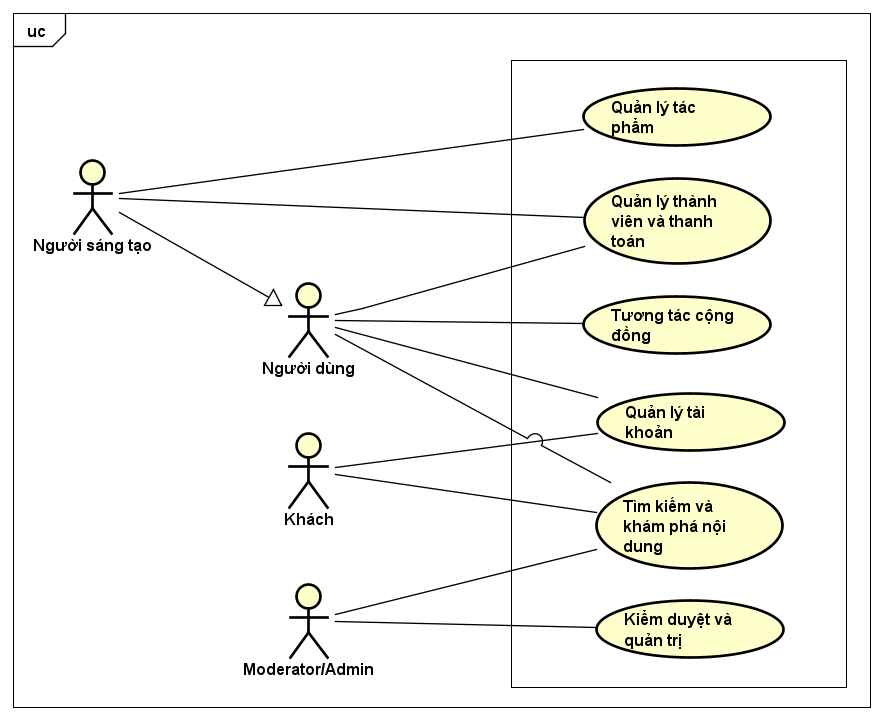
\includegraphics[width=0.65\linewidth]{Hinh_2_1_Use_case_tong_quat.png}
\caption{Biểu đồ use case tổng quát của hệ thống}
\label{fig:2_1}
\end{figure}
\FloatBarrier

Các use case mức cao của hệ thống gồm: quản lý tài khoản, quản lý tác phẩm, tìm kiếm và khám phá nội dung, tương tác cộng đồng, quản lý thành viên và thanh toán, kiểm duyệt và quản trị. Nhóm quản lý tài khoản bao phủ đăng nhập, đồng bộ hồ sơ, cập nhật thông tin cá nhân và trở thành người sáng tạo. Nhóm quản lý tác phẩm bao phủ đăng tải, xử lý ảnh, chỉnh sửa, xem trạng thái và quản lý quyền truy cập theo tier. Nhóm tìm kiếm và khám phá bao phủ tìm kiếm toàn văn, lọc, sắp xếp, tìm kiếm ngữ nghĩa, tìm kiếm bằng phác thảo và gợi ý nội dung. Nhóm tương tác cộng đồng bao phủ thích, bình luận, lưu vào bộ sưu tập, theo dõi và báo cáo vi phạm. Nhóm thành viên và thanh toán bao phủ plan nền tảng, artist tier, đăng ký, hủy đăng ký, lịch sử thanh toán, doanh thu và payout. Nhóm kiểm duyệt và quản trị bao phủ xử lý report, appeal, duyệt hoặc từ chối tác phẩm, quản lý người dùng, audit log và thống kê.

\subsection{Biểu đồ use case phân rã Quản lý tài khoản}
\label{subsection:2.2.2}

Use case Quản lý tài khoản liên quan đến cả người dùng thường và người sáng tạo. Hệ thống sử dụng Clerk cho xác thực, nhưng vẫn duy trì hồ sơ người dùng nội bộ để lưu vai trò, trạng thái artist, trạng thái bị khóa, thông tin Stripe và các quan hệ xã hội. Khi người dùng đăng nhập lần đầu, backend thực hiện đồng bộ lười, tạo hoặc cập nhật bản ghi người dùng dựa trên định danh Clerk.

\begin{figure}[h!]
\centering
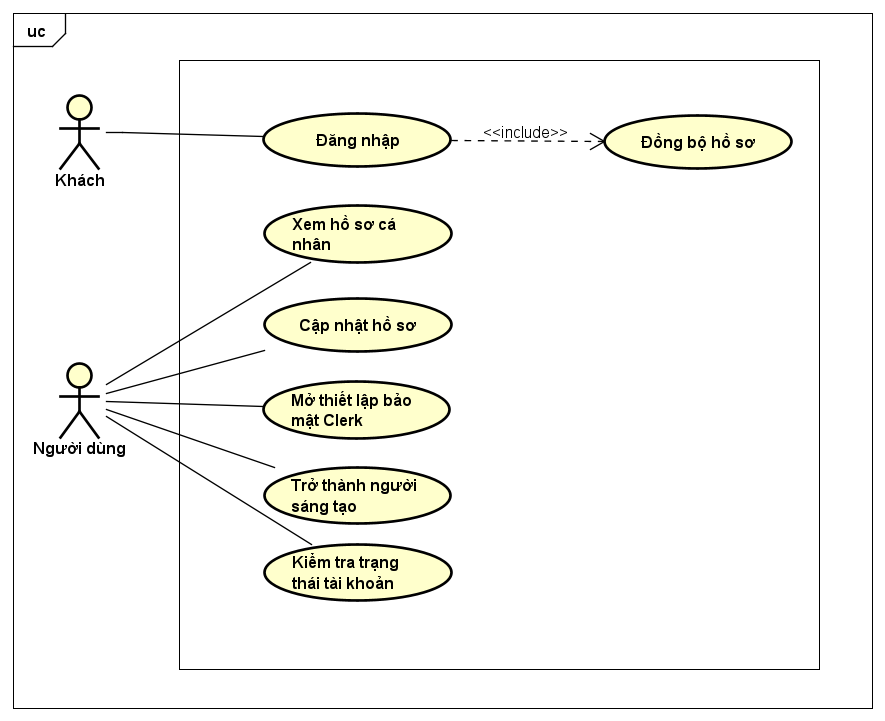
\includegraphics[width=0.58\linewidth]{Hinh_2_2_Use_case_Quan_ly_tai_khoan.png}
\caption{Biểu đồ use case phân rã Quản lý tài khoản}
\label{fig:2_2}
\end{figure}
\FloatBarrier

Các use case con gồm đăng nhập, xem hồ sơ cá nhân, cập nhật hồ sơ, mở trang thiết lập bảo mật của Clerk, trở thành người sáng tạo, xem dashboard cá nhân và kiểm tra trạng thái tài khoản. Đối với người dùng bị khóa, middleware phía frontend gọi backend để kiểm tra trạng thái và chuyển hướng người dùng sang trang thông báo chặn nếu cần.

\subsection{Biểu đồ use case phân rã Quản lý tác phẩm}
\label{subsection:2.2.3}

Use case Quản lý tác phẩm là trung tâm của hệ thống. Người sáng tạo có thể đăng tải một tác phẩm gồm một hoặc nhiều ảnh, nhập tiêu đề, mô tả, tag, chọn visibility, chọn tier yêu cầu nếu là nội dung giới hạn, cấu hình watermark và theo dõi trạng thái xử lý. Sau khi tạo tác phẩm, hệ thống đưa tác phẩm vào hàng đợi để worker xử lý ảnh bất đồng bộ.

\begin{figure}[h!]
\centering
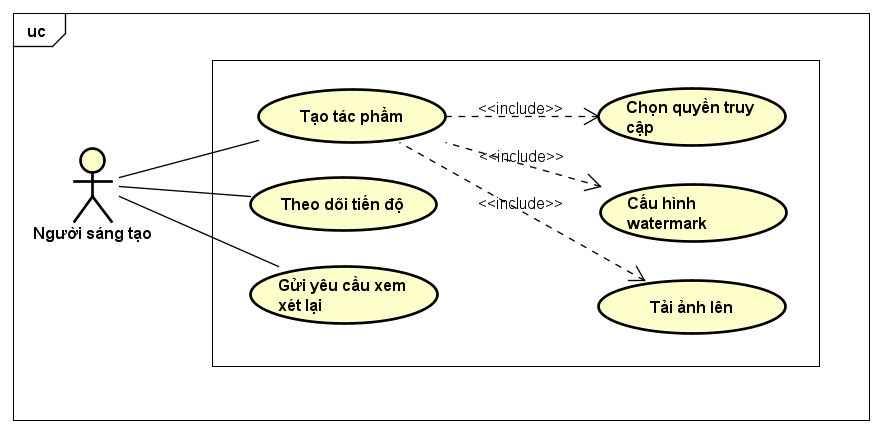
\includegraphics[width=0.58\linewidth]{Hinh_2_3_Use_case_Quan_ly_tac_pham.png}
\caption{Biểu đồ use case phân rã Quản lý tác phẩm}
\label{fig:2_3}
\end{figure}
\FloatBarrier

Các use case con gồm tạo tác phẩm, tải ảnh lên, cấu hình watermark, chọn quyền truy cập, gửi xử lý nền, xem tiến độ xử lý, xem tác phẩm đã xuất bản, chỉnh sửa thông tin, quảng bá tác phẩm, xem tác phẩm liên quan và gửi appeal khi tác phẩm bị đưa vào trạng thái cần xử lý. Hệ thống phân biệt trạng thái tác phẩm như đang xử lý, đã xuất bản, thất bại, cần xử lý và đang được xem xét lại. Thiết kế này phù hợp với thực tế xử lý ảnh vì kiểm duyệt và phát hiện trùng lặp có thể xảy ra ở từng ảnh trong cùng một tác phẩm.

\subsection{Biểu đồ use case phân rã Tìm kiếm và khám phá nội dung}
\label{subsection:2.2.4}

Use case Tìm kiếm và khám phá nội dung phục vụ cả khách và người dùng đã đăng nhập. Khách có thể tìm kiếm và xem nội dung công khai; người dùng đã đăng nhập có thêm khả năng tìm kiếm cá nhân hóa, dùng tìm kiếm bằng phác thảo nếu thỏa điều kiện gói dịch vụ và nhận gợi ý dựa trên lịch sử tương tác.

\begin{figure}[h!]
\centering
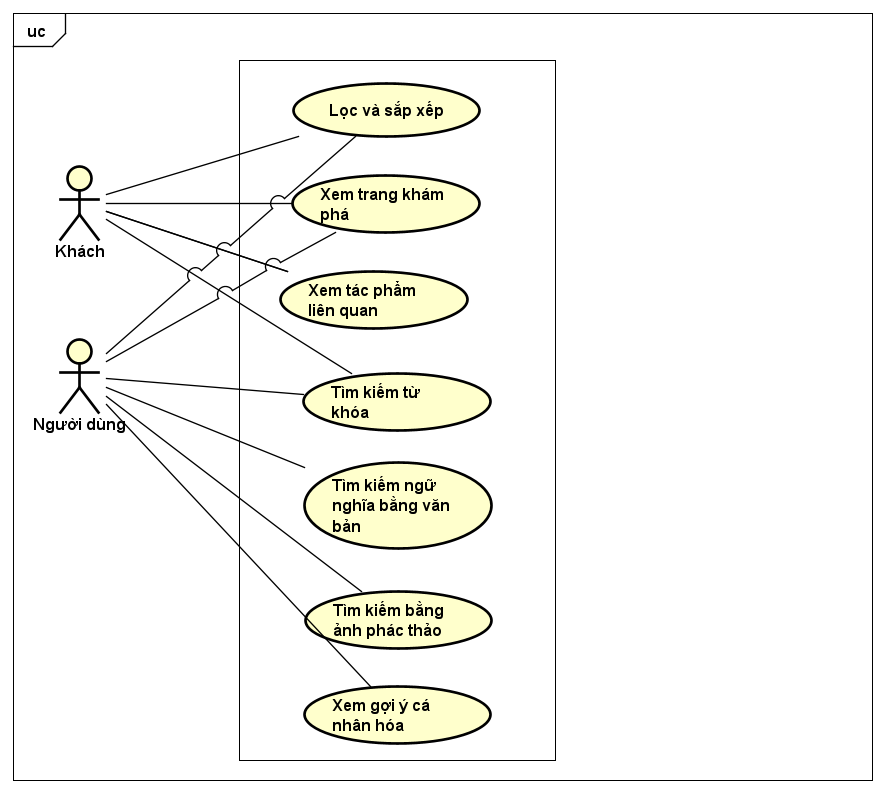
\includegraphics[width=0.58\linewidth]{Hinh_2_4_Use_case_Tim_kiem_kham_pha.png}
\caption{Biểu đồ use case phân rã Tìm kiếm và khám phá nội dung}
\label{fig:2_4}
\end{figure}
\FloatBarrier

Các use case con gồm tìm kiếm theo từ khóa, lọc theo tag, tỷ lệ ảnh, độ phân giải và nội dung AI, sắp xếp theo thời gian hoặc độ phổ biến, tìm kiếm ngữ nghĩa bằng văn bản, tìm kiếm bằng ảnh phác thảo, xem trang khám phá, xem tác phẩm phổ biến, xem nghệ sĩ nổi bật, xem tag thịnh hành và xem gợi ý tác phẩm liên quan. Hệ thống sử dụng Meilisearch cho tìm kiếm toàn văn và pgvector cho tìm kiếm ngữ nghĩa.

\subsection{Biểu đồ use case phân rã Tương tác cộng đồng}
\label{subsection:2.2.5}

Use case Tương tác cộng đồng bao phủ các hành vi giúp người dùng hình thành quan hệ xã hội xung quanh tác phẩm. Đây là nhóm chức năng làm cho nền tảng không chỉ là kho lưu trữ ảnh mà trở thành cộng đồng.

\begin{figure}[h!]
\centering
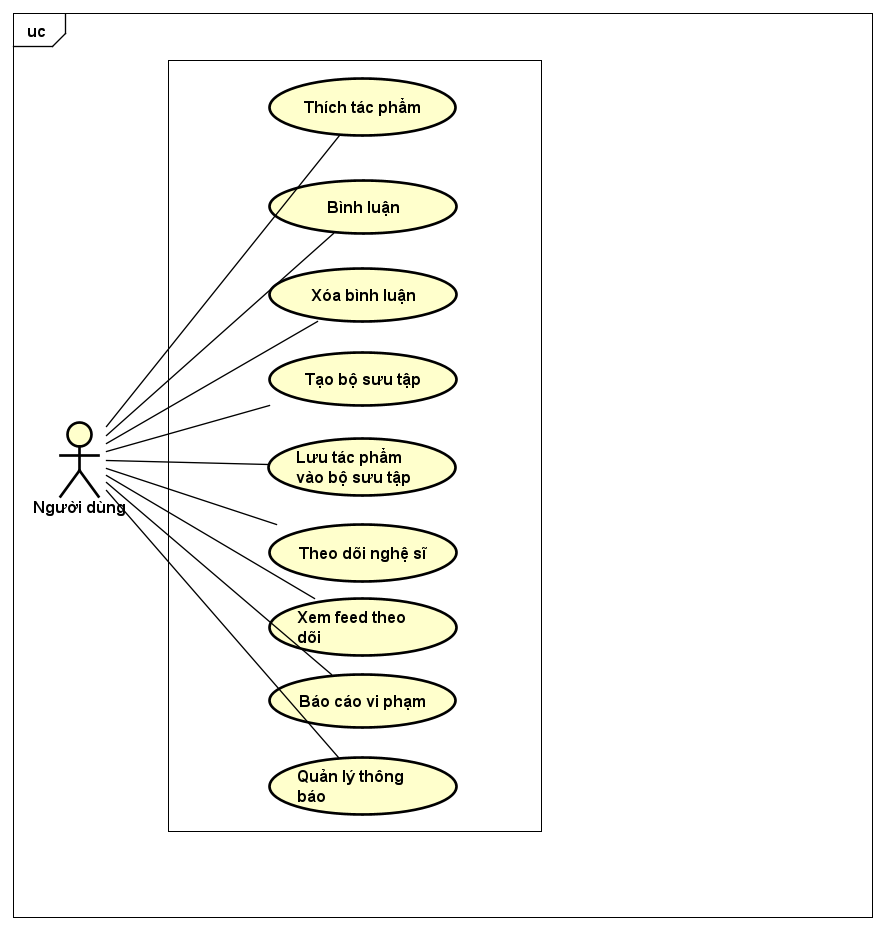
\includegraphics[width=0.58\linewidth]{Hinh_2_5_Use_case_Tuong_tac_cong_dong.png}
\caption{Biểu đồ use case phân rã Tương tác cộng đồng}
\label{fig:2_5}
\end{figure}
\FloatBarrier

Các use case con gồm thích hoặc bỏ thích tác phẩm, bình luận, xóa bình luận của bản thân, lưu tác phẩm vào collection, tạo collection, thêm hoặc xóa tác phẩm khỏi collection, theo dõi hoặc bỏ theo dõi nghệ sĩ, xem feed theo dõi, báo cáo tác phẩm vi phạm và nhận thông báo. Một số tương tác như lượt xem hoặc lượt thích cũng được dùng để cập nhật thống kê và đồng bộ sang chỉ mục tìm kiếm.

\subsection{Biểu đồ use case phân rã Quản lý thành viên và thanh toán}
\label{subsection:2.2.6}

Use case Quản lý thành viên và thanh toán bao gồm hai nhánh: subscription nền tảng và subscription theo artist tier. Subscription nền tảng phục vụ các quyền lợi chung của người dùng, còn artist tier phục vụ quan hệ trả phí giữa người sáng tạo và người hâm mộ.

\begin{figure}[h!]
\centering
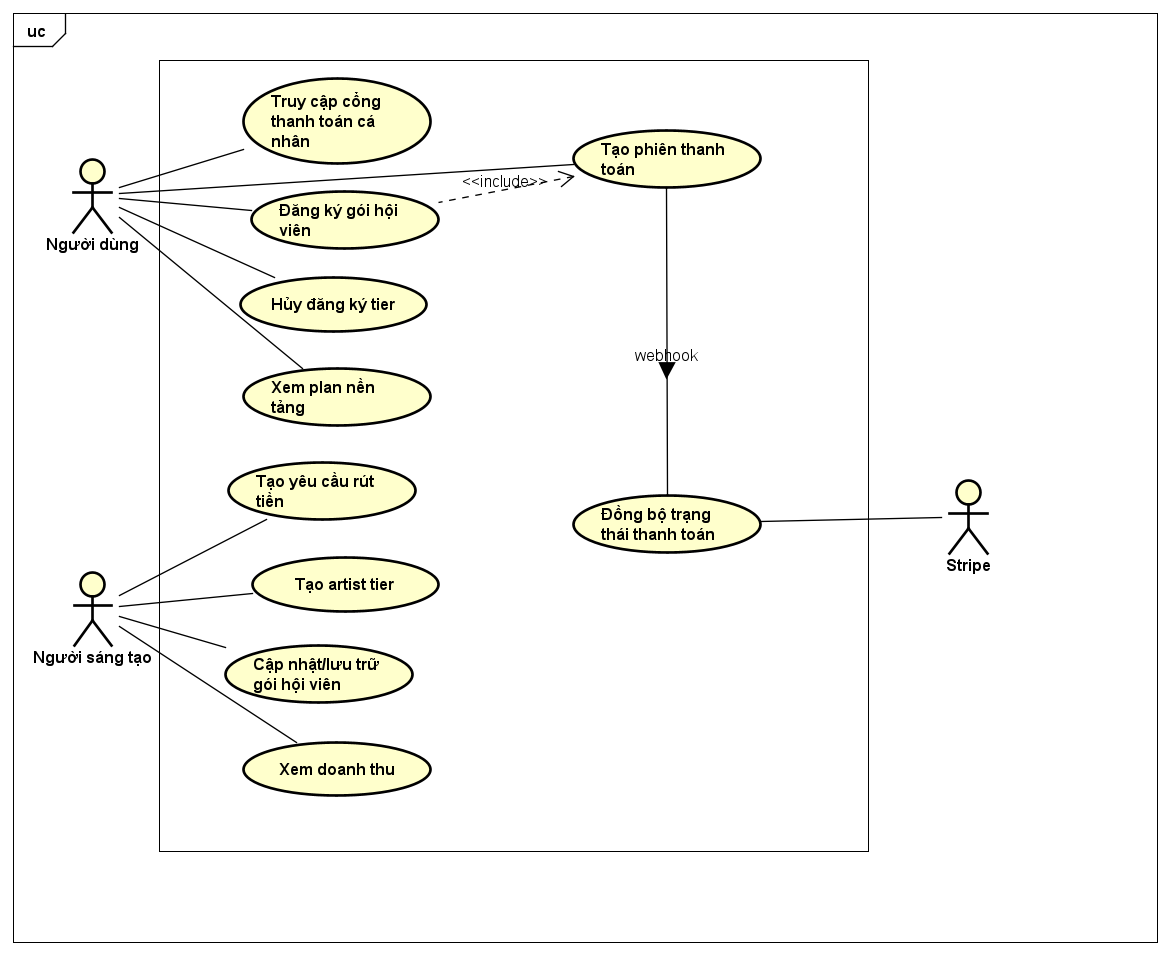
\includegraphics[width=0.58\linewidth]{Hinh_2_6_Use_case_Thanh_vien_thanh_toan.png}
\caption{Biểu đồ use case phân rã Quản lý thành viên và thanh toán}
\label{fig:2_6}
\end{figure}
\FloatBarrier

Các use case con gồm xem danh sách plan, tạo phiên thanh toán, đồng bộ kết quả checkout, mở customer portal, hủy subscription, tạo artist tier, cập nhật artist tier, archive tier, xem danh sách người đăng ký tier, đăng ký tier của artist, hủy đăng ký tier, xem lịch sử thanh toán, xem doanh thu và tạo yêu cầu payout. Hệ thống tích hợp cổng thanh toán (Stripe/PayPal) để xử lý thanh toán và webhook để đồng bộ trạng thái về cơ sở dữ liệu nội bộ.

\subsection{Biểu đồ use case phân rã Kiểm duyệt và quản trị}
\label{subsection:2.2.7}

Use case Kiểm duyệt và quản trị dành cho Moderator, Admin và Super Admin. Đây là nhóm chức năng đảm bảo nền tảng vận hành an toàn, kiểm soát được nội dung vi phạm và truy vết được thao tác quan trọng.

\begin{figure}[h!]
\centering
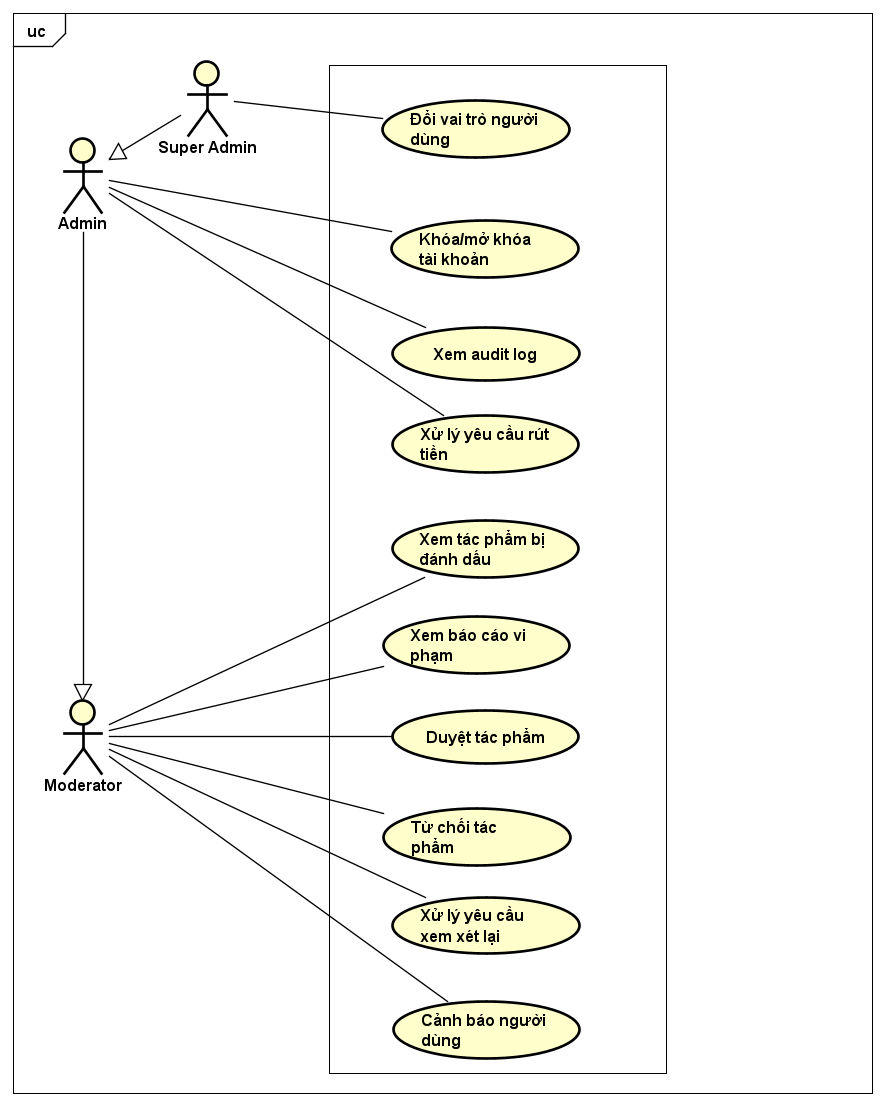
\includegraphics[width=0.58\linewidth]{Hinh_2_7_Use_case_Kiem_duyet_quan_tri.png}
\caption{Biểu đồ use case phân rã Kiểm duyệt và quản trị}
\label{fig:2_7}
\end{figure}
\FloatBarrier

Các use case con gồm xem danh sách tác phẩm bị đánh dấu, xem báo cáo vi phạm của tác phẩm, duyệt tác phẩm, từ chối tác phẩm, xử lý yêu cầu xem xét lại, xem lịch sử report đã giải quyết, cảnh báo người dùng, khóa hoặc mở khóa người dùng, thay đổi vai trò người dùng, xem thống kê dashboard, cấu hình trọng số xếp hạng, cấu hình tìm kiếm khám phá, xem audit log, quản lý nhân sự điều phối và xử lý yêu cầu rút tiền. Hệ thống cần đảm bảo chỉ người có vai trò phù hợp mới truy cập được các chức năng này.

\subsection{Quy trình nghiệp vụ}
\label{subsection:2.2.8}

Quy trình nghiệp vụ quan trọng nhất của hệ thống là quy trình đăng tải và xử lý tác phẩm. Quy trình này kết hợp nhiều use case: đăng nhập, tạo tác phẩm, tải ảnh, đưa job vào hàng đợi, xử lý ảnh, kiểm tra trùng lặp, kiểm duyệt NSFW, lưu biến thể ảnh, lập chỉ mục tìm kiếm, sinh embedding và thông báo kết quả cho người sáng tạo.

\begin{figure}[h!]
\centering
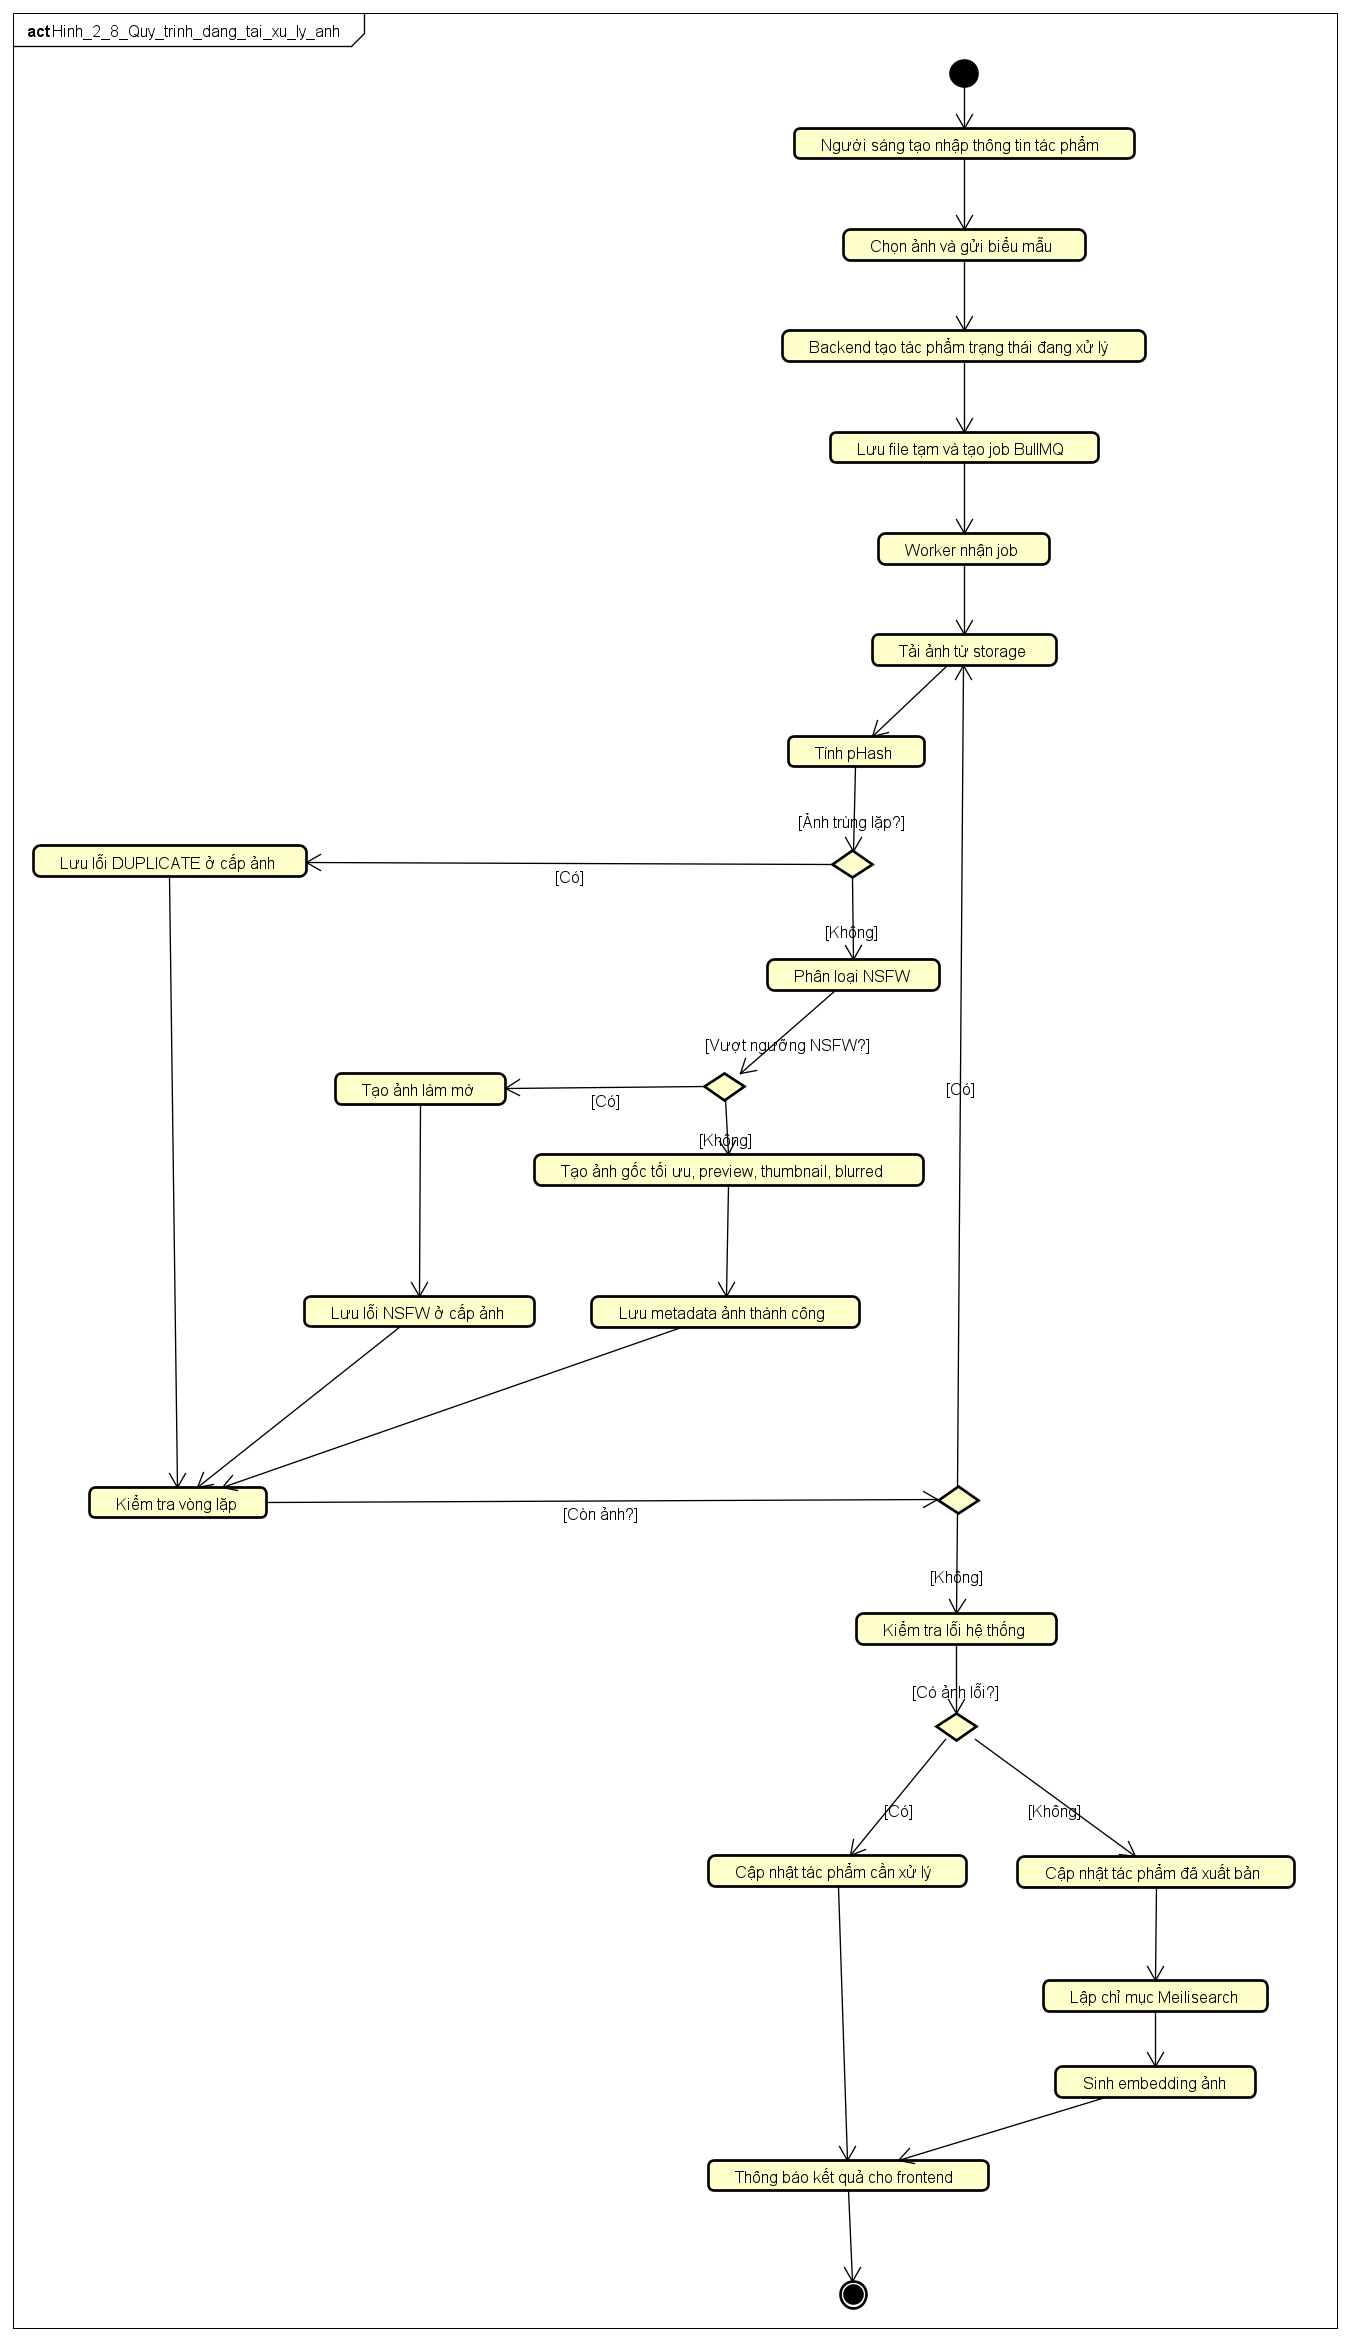
\includegraphics[width=0.65\linewidth]{Hinh_2_8_Quy_trinh_dang_tai_xu_ly_anh.png}
\caption{Quy trình nghiệp vụ đăng tải và xử lý tác phẩm}
\label{fig:2_8}
\end{figure}
\FloatBarrier

Mô tả sơ bộ quy trình như sau. Người sáng tạo đăng nhập và truy cập trang upload. Sau khi nhập thông tin tác phẩm và chọn ảnh, frontend gửi yêu cầu tạo tác phẩm tới backend. Backend lưu metadata, lưu tệp tạm vào storage, tạo job xử lý ảnh và trả về mã job cho frontend theo dõi. Worker nhận job, tải từng ảnh, tính pHash để phát hiện trùng lặp, phân loại NSFW, tạo ảnh gốc tối ưu, ảnh xem trước, ảnh thu nhỏ và ảnh làm mờ. Nếu ảnh hợp lệ, thông tin ảnh được lưu với trạng thái thành công; nếu ảnh trùng lặp hoặc nhạy cảm, hệ thống lưu metadata lỗi ở cấp ảnh. Khi tất cả ảnh đã được xử lý, nếu không có lỗi, tác phẩm được xuất bản và lập chỉ mục tìm kiếm; nếu có lỗi, tác phẩm chuyển sang trạng thái cần xử lý để người sáng tạo hoặc quản trị viên xem xét.

Quy trình nghiệp vụ thứ hai là quy trình đăng ký artist tier. Quy trình này kết hợp các use case xem tier công khai, tạo phiên thanh toán, thanh toán qua cổng thanh toán, webhook đồng bộ subscription và kiểm tra quyền truy cập nội dung giới hạn.

\begin{figure}[h!]
\centering
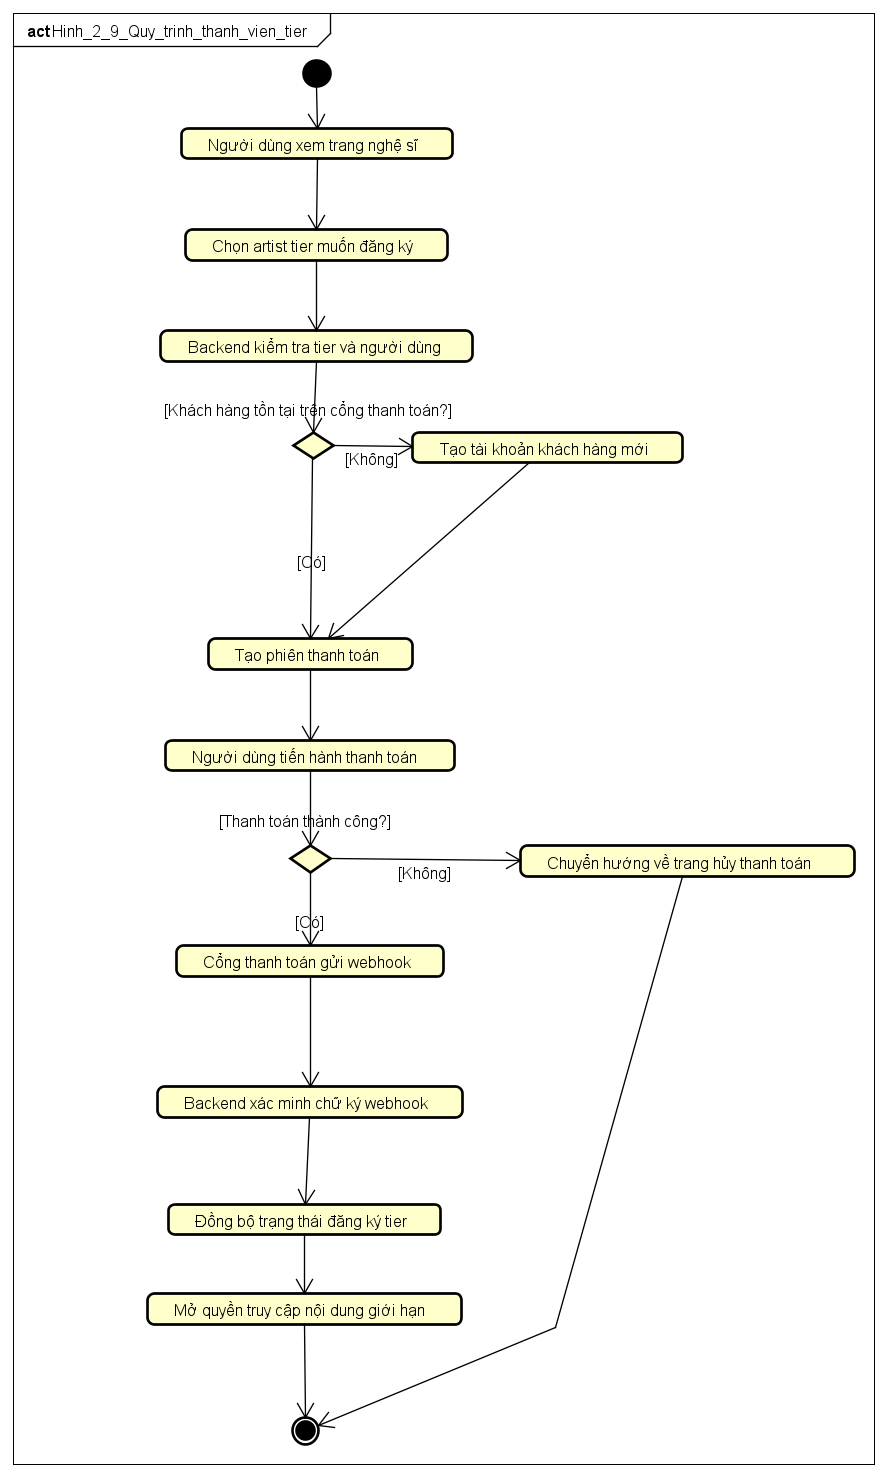
\includegraphics[width=0.65\linewidth]{Hinh_2_9_Quy_trinh_thanh_vien_tier.png}
\caption{Quy trình nghiệp vụ đăng ký gói thành viên của người sáng tạo}
\label{fig:2_9}
\end{figure}
\FloatBarrier

Người dùng truy cập trang nghệ sĩ và xem các tier đang hoạt động. Khi chọn đăng ký một tier, backend kiểm tra người dùng, đảm bảo khách hàng trên cổng thanh toán tồn tại và tạo phiên thanh toán. Sau khi người dùng thanh toán, cổng thanh toán gửi webhook về backend. Backend xác minh chữ ký webhook, đọc metadata của subscription, cập nhật bảng đăng ký tier và ghi nhận thanh toán. Từ thời điểm subscription ở trạng thái hoạt động, người dùng được phép truy cập các tác phẩm đặt quyền truy cập theo tier tương ứng.

\clearpage
\section{Đặc tả chức năng}
\label{section:2.3}

Phần này đặc tả sáu use case quan trọng của hệ thống. Mỗi use case được trình bày theo cấu trúc gồm mã use case, tên use case, tác nhân, tiền điều kiện, tóm tắt, luồng sự kiện chính, luồng sự kiện thay thế và hậu điều kiện. Các use case được lựa chọn là những chức năng có ảnh hưởng lớn tới kiến trúc và nghiệp vụ của hệ thống.

\subsection{Đặc tả use case Đăng nhập và đồng bộ tài khoản}
\label{subsection:2.3.1}

\begin{table}[h!]
\centering
\small
\renewcommand{\arraystretch}{1.2}
\begin{tabular}{|p{0.24\linewidth}|p{0.68\linewidth}|}
\hline
\textbf{Use Case ID} & UC-01 \\
\hline
\textbf{Tên Use Case} & Đăng nhập và đồng bộ tài khoản \\
\hline
\textbf{Tác nhân} & Khách, Người dùng \\
\hline
\textbf{Tiền điều kiện} & Người dùng có tài khoản hợp lệ trên dịch vụ xác thực Clerk hoặc có khả năng đăng ký tài khoản mới. \\
\hline
\textbf{Tóm tắt} & Người dùng đăng nhập vào hệ thống. Backend xác minh token Clerk và tạo hoặc cập nhật hồ sơ người dùng trong cơ sở dữ liệu nội bộ. \\
\hline
\textbf{Luồng sự kiện chính} &
1. Khách truy cập trang đăng nhập. \newline
2. Hệ thống hiển thị giao diện đăng nhập của Clerk. \newline
3. Người dùng nhập thông tin xác thực hoặc chọn phương thức đăng nhập hỗ trợ. \newline
4. Clerk xác thực thành công và cấp phiên đăng nhập. \newline
5. Frontend gọi API cần xác thực kèm token. \newline
6. Backend xác minh token, lấy định danh Clerk của người dùng. \newline
7. Backend tìm bản ghi người dùng theo định danh Clerk. \newline
8. Nếu bản ghi chưa tồn tại, backend tạo hồ sơ người dùng mới gồm email, username, tên hiển thị và avatar. \newline
9. Hệ thống trả về thông tin người dùng nội bộ cho frontend. \\
\hline
\textbf{Luồng sự kiện thay thế} &
\textbf{Thông tin xác thực không hợp lệ:} Clerk từ chối đăng nhập và yêu cầu người dùng nhập lại thông tin. \newline
\textbf{Tài khoản bị khóa:} Sau khi xác thực, frontend gọi API kiểm tra hồ sơ; nếu người dùng bị khóa, hệ thống chuyển hướng sang trang thông báo chặn. \newline
\textbf{Lỗi đồng bộ hồ sơ:} Backend trả về lỗi, frontend hiển thị thông báo và yêu cầu người dùng thử lại. \\
\hline
\textbf{Hậu điều kiện} & Người dùng có phiên đăng nhập hợp lệ; cơ sở dữ liệu nội bộ có bản ghi người dùng tương ứng với định danh Clerk. \\
\hline
\end{tabular}
    \caption{Đặc tả use case Đăng nhập và đồng bộ tài khoản}
    \label{table:2_2}

\end{table}
\FloatBarrier

\subsection{Đặc tả use case Đăng tải tác phẩm}
\label{subsection:2.3.2}

\begin{table}[h!]
\centering
\small
\renewcommand{\arraystretch}{1.2}
\begin{tabular}{|p{0.24\linewidth}|p{0.68\linewidth}|}
\hline
\textbf{Use Case ID} & UC-02 \\
\hline
\textbf{Tên Use Case} & Đăng tải tác phẩm \\
\hline
\textbf{Tác nhân} & Người sáng tạo \\
\hline
\textbf{Tiền điều kiện} & Người dùng đã đăng nhập, không bị khóa tài khoản và có quyền đăng tải tác phẩm. \\
\hline
\textbf{Tóm tắt} & Người sáng tạo tạo tác phẩm mới, tải lên một hoặc nhiều ảnh. Hệ thống xử lý ảnh qua hàng đợi nền, kiểm tra trùng lặp, kiểm duyệt NSFW và xuất bản nếu hợp lệ. \\
\hline
\textbf{Luồng sự kiện chính} &
1. Người sáng tạo truy cập trang upload. \newline
2. Hệ thống hiển thị biểu mẫu tạo tác phẩm. \newline
3. Người sáng tạo nhập tiêu đề, mô tả, tag, loại tác phẩm, trạng thái AI, quyền truy cập và cấu hình watermark nếu có. \newline
4. Người sáng tạo chọn một hoặc nhiều ảnh và gửi biểu mẫu. \newline
5. Backend kiểm tra dữ liệu đầu vào và tạo bản ghi tác phẩm ở trạng thái đang xử lý. \newline
6. Backend lưu tệp ảnh tạm và tạo job xử lý ảnh trong hàng đợi. \newline
7. Worker tải ảnh, tính pHash, kiểm tra trùng lặp, phân loại NSFW, tạo các biến thể ảnh và lưu metadata ảnh. \newline
8. Nếu tất cả ảnh hợp lệ, hệ thống cập nhật tác phẩm sang trạng thái đã xuất bản. \newline
9. Hệ thống lập chỉ mục tác phẩm vào Meilisearch và sinh embedding cho ảnh. \newline
10. Frontend hiển thị thông báo xử lý hoàn tất. \\
\hline
\textbf{Luồng sự kiện thay thế} &
\textbf{Dữ liệu nhập không hợp lệ:} Backend trả về lỗi validation, frontend yêu cầu người dùng sửa biểu mẫu. \newline
\textbf{Ảnh bị trùng lặp:} Worker lưu metadata lỗi ở cấp ảnh, tác phẩm chuyển sang trạng thái cần xử lý. \newline
\textbf{Ảnh bị phát hiện NSFW:} Worker tạo ảnh làm mờ, lưu điểm phát hiện và chuyển tác phẩm sang trạng thái cần xử lý. \newline
\textbf{Lỗi xử lý ảnh:} Tác phẩm chuyển sang trạng thái thất bại, hệ thống ghi log phục vụ điều tra. \\
\hline
\textbf{Hậu điều kiện} & Tác phẩm được xuất bản nếu hợp lệ; nếu có lỗi, tác phẩm được lưu ở trạng thái cần xử lý hoặc thất bại để người dùng và quản trị viên theo dõi. \\
\hline
\end{tabular}
    \caption{Đặc tả use case Đăng tải tác phẩm}
    \label{table:2_3}

\end{table}
\FloatBarrier

\subsection{Đặc tả use case Tìm kiếm và khám phá tác phẩm}
\label{subsection:2.3.3}

\begin{table}[h!]
\centering
\small
\renewcommand{\arraystretch}{1.2}
\begin{tabular}{|p{0.24\linewidth}|p{0.68\linewidth}|}
\hline
\textbf{Use Case ID} & UC-03 \\
\hline
\textbf{Tên Use Case} & Tìm kiếm và khám phá tác phẩm \\
\hline
\textbf{Tác nhân} & Khách, Người dùng \\
\hline
\textbf{Tiền điều kiện} & Hệ thống có dữ liệu tác phẩm đã xuất bản và chỉ mục tìm kiếm đã được cập nhật. \\
\hline
\textbf{Tóm tắt} & Tác nhân tìm kiếm tác phẩm theo từ khóa, tag, bộ lọc, truy vấn ngữ nghĩa hoặc ảnh phác thảo. \\
\hline
\textbf{Luồng sự kiện chính} &
1. Tác nhân truy cập trang tìm kiếm hoặc khám phá. \newline
2. Hệ thống hiển thị ô tìm kiếm, bộ lọc và danh sách nội dung ban đầu. \newline
3. Tác nhân nhập từ khóa hoặc chọn bộ lọc như tag, tỷ lệ ảnh, độ phân giải, nội dung AI và cách sắp xếp. \newline
4. Frontend gửi truy vấn tới backend. \newline
5. Backend truy vấn Meilisearch đối với tìm kiếm toàn văn hoặc truy vấn pgvector đối với tìm kiếm ngữ nghĩa. \newline
6. Backend trả về danh sách tác phẩm phù hợp cùng thông tin tác giả, thumbnail, tag và chỉ số tương tác. \newline
7. Frontend hiển thị kết quả và cho phép tác nhân mở trang chi tiết tác phẩm. \\
\hline
\textbf{Luồng sự kiện thay thế} &
\textbf{Không có kết quả:} Hệ thống hiển thị thông báo không tìm thấy kết quả phù hợp và gợi ý thay đổi bộ lọc. \newline
\textbf{Tìm kiếm ngữ nghĩa chưa khả dụng:} Nếu dịch vụ embedding chưa sẵn sàng, hệ thống trả về thông báo và có thể gợi ý dùng tìm kiếm từ khóa. \newline
\textbf{Người dùng vượt giới hạn tìm kiếm miễn phí:} Hệ thống từ chối truy vấn theo chính sách giới hạn và gợi ý nâng cấp gói. \\
\hline
\textbf{Hậu điều kiện} & Danh sách kết quả phù hợp được hiển thị; các truy vấn ngữ nghĩa có thể được cache để tăng hiệu năng cho lần sau. \\
\hline
\end{tabular}
    \caption{Đặc tả use case Tìm kiếm và khám phá tác phẩm}
    \label{table:2_4}

\end{table}
\FloatBarrier

\subsection{Đặc tả use case Tương tác với tác phẩm}
\label{subsection:2.3.4}

\begin{table}[h!]
\centering
\small
\renewcommand{\arraystretch}{1.2}
\begin{tabular}{|p{0.24\linewidth}|p{0.68\linewidth}|}
\hline
\textbf{Use Case ID} & UC-04 \\
\hline
\textbf{Tên Use Case} & Tương tác với tác phẩm \\
\hline
\textbf{Tác nhân} & Người dùng \\
\hline
\textbf{Tiền điều kiện} & Người dùng đã đăng nhập; tác phẩm tồn tại và người dùng có quyền xem tác phẩm. \\
\hline
\textbf{Tóm tắt} & Người dùng thích, bình luận, lưu vào bộ sưu tập, theo dõi tác giả hoặc báo cáo tác phẩm vi phạm. \\
\hline
\textbf{Luồng sự kiện chính} &
1. Người dùng mở trang chi tiết tác phẩm. \newline
2. Hệ thống kiểm tra quyền truy cập đối với tác phẩm công khai hoặc tác phẩm giới hạn theo tier. \newline
3. Người dùng chọn một hành động tương tác: thích, bình luận, lưu vào collection hoặc theo dõi tác giả. \newline
4. Backend xác thực người dùng và kiểm tra điều kiện nghiệp vụ của hành động. \newline
5. Backend ghi nhận tương tác trong cơ sở dữ liệu. \newline
6. Hệ thống cập nhật bộ đếm liên quan như lượt thích, bình luận hoặc trạng thái lưu. \newline
7. Frontend cập nhật giao diện để phản ánh kết quả. \\
\hline
\textbf{Luồng sự kiện thay thế} &
\textbf{Người dùng chưa có quyền xem:} Hệ thống yêu cầu đăng nhập hoặc đăng ký tier phù hợp. \newline
\textbf{Bình luận không hợp lệ:} Backend từ chối nội dung rỗng hoặc không thỏa quy định. \newline
\textbf{Báo cáo vi phạm:} Người dùng chọn lý do, gửi mô tả; hệ thống tạo report để quản trị viên xử lý. \newline
\textbf{Thao tác trùng lặp:} Nếu người dùng đã thích hoặc đã lưu, hệ thống chuyển hành động thành bỏ thích hoặc bỏ lưu tùy ngữ cảnh. \\
\hline
\textbf{Hậu điều kiện} & Tương tác được ghi nhận; bộ đếm và trạng thái giao diện được cập nhật; nếu có report, report được đưa vào hàng xử lý kiểm duyệt. \\
\hline
\end{tabular}
    \caption{Đặc tả use case Tương tác với tác phẩm}
    \label{table:2_5}

\end{table}
\FloatBarrier

\subsection{Đặc tả use case Đăng ký gói thành viên của người sáng tạo}
\label{subsection:2.3.5}

\begin{table}[h!]
\centering
\small
\renewcommand{\arraystretch}{1.2}
\begin{tabular}{|p{0.24\linewidth}|p{0.68\linewidth}|}
\hline
\textbf{Use Case ID} & UC-05 \\
\hline
\textbf{Tên Use Case} & Đăng ký gói thành viên của người sáng tạo \\
\hline
\textbf{Tác nhân} & Người dùng, Người sáng tạo, Cổng thanh toán \\
\hline
\textbf{Tiền điều kiện} & Người dùng đã đăng nhập; người sáng tạo có ít nhất một artist tier đang hoạt động; Cổng thanh toán được cấu hình hợp lệ. \\
\hline
\textbf{Tóm tắt} & Người dùng đăng ký một tier của người sáng tạo để truy cập nội dung giới hạn và quyền lợi tương ứng. \\
\hline
\textbf{Luồng sự kiện chính} &
1. Người dùng truy cập trang nghệ sĩ hoặc trang membership. \newline
2. Hệ thống hiển thị danh sách artist tier công khai. \newline
3. Người dùng chọn tier muốn đăng ký. \newline
4. Backend kiểm tra tier, người dùng và khách hàng trên cổng thanh toán. \newline
5. Backend tạo phiên thanh toán và trả về đường dẫn checkout. \newline
6. Người dùng hoàn tất thanh toán trên cổng thanh toán. \newline
7. cổng thanh toán gửi webhook về backend. \newline
8. Backend xác minh webhook và đồng bộ trạng thái tier subscription. \newline
9. Hệ thống cho phép người dùng truy cập nội dung giới hạn theo tier đã đăng ký. \\
\hline
\textbf{Luồng sự kiện thay thế} &
\textbf{Người dùng hủy thanh toán:} Cổng thanh toán chuyển người dùng về trang hủy, subscription không được kích hoạt. \newline
\textbf{Webhook không hợp lệ:} Backend từ chối sự kiện và ghi log lỗi. \newline
\textbf{Tier bị archive hoặc không tồn tại:} Backend từ chối tạo checkout session. \newline
\textbf{Subscription quá hạn hoặc bị hủy:} Người dùng mất quyền truy cập nội dung giới hạn sau khi hệ thống đồng bộ trạng thái. \\
\hline
\textbf{Hậu điều kiện} & Nếu thanh toán thành công, subscription nội bộ ở trạng thái hoạt động và quyền truy cập nội dung giới hạn được mở cho người dùng. \\
\hline
\end{tabular}
    \caption{Đặc tả use case Đăng ký gói thành viên của người sáng tạo}
    \label{table:2_6}

\end{table}
\FloatBarrier

\subsection{Đặc tả use case Kiểm duyệt báo cáo và appeal}
\label{subsection:2.3.6}

\begin{table}[h!]
\centering
\small
\renewcommand{\arraystretch}{1.2}
\begin{tabular}{|p{0.24\linewidth}|p{0.68\linewidth}|}
\hline
\textbf{Use Case ID} & UC-06 \\
\hline
\textbf{Tên Use Case} & Kiểm duyệt báo cáo và appeal \\
\hline
\textbf{Tác nhân} & Người dùng, Người sáng tạo, Moderator, Admin \\
\hline
\textbf{Tiền điều kiện} & Có tác phẩm bị báo cáo, bị hệ thống đánh dấu hoặc được người sáng tạo gửi appeal; quản trị viên đã đăng nhập và có quyền xử lý. \\
\hline
\textbf{Tóm tắt} & Điều phối viên xem xét báo cáo hoặc appeal, sau đó duyệt, từ chối, cảnh báo hoặc áp dụng biện pháp xử lý đối với tác phẩm và người dùng liên quan. \\
\hline
\textbf{Luồng sự kiện chính} &
1. Moderator hoặc Admin truy cập trang kiểm duyệt. \newline
2. Hệ thống hiển thị danh sách tác phẩm bị đánh dấu hoặc report đang chờ xử lý. \newline
3. Điều phối viên mở chi tiết tác phẩm, xem ảnh, metadata lỗi, pHash liên quan, report và lịch sử xử lý. \newline
4. Điều phối viên đưa ra quyết định duyệt hoặc từ chối. \newline
5. Backend cập nhật trạng thái tác phẩm và trạng thái report. \newline
6. Nếu cần, backend tạo cảnh báo cho người dùng hoặc cập nhật trạng thái khóa tài khoản. \newline
7. Hệ thống ghi audit log cho thao tác quản trị. \newline
8. Người sáng tạo hoặc người báo cáo nhận được kết quả xử lý qua giao diện hoặc thông báo. \\
\hline
\textbf{Luồng sự kiện thay thế} &
\textbf{Người sáng tạo gửi appeal:} Nếu tác phẩm ở trạng thái cần xử lý, hệ thống chuyển tác phẩm sang trạng thái đang xem xét lại. \newline
\textbf{Bằng chứng chưa đủ:} Điều phối viên có thể giữ report ở trạng thái chờ xử lý hoặc yêu cầu thông tin bổ sung. \newline
\textbf{Người dùng vi phạm nhiều lần:} Điều phối viên có thể cảnh báo, khóa tạm thời hoặc khóa dài hạn tùy mức độ. \newline
\textbf{Không đủ quyền:} Backend từ chối yêu cầu nếu tài khoản không có vai trò phù hợp. \\
\hline
\textbf{Hậu điều kiện} & Report được cập nhật trạng thái; tác phẩm được duyệt, từ chối hoặc tiếp tục chờ xử lý; thao tác quản trị được ghi nhận trong audit log. \\
\hline
\end{tabular}
    \caption{Đặc tả use case Kiểm duyệt báo cáo và appeal}
    \label{table:2_7}

\end{table}
\FloatBarrier

\section{Yêu cầu phi chức năng}
\label{section:2.4}

Bên cạnh yêu cầu chức năng, hệ thống cần đáp ứng các yêu cầu phi chức năng để có thể vận hành ổn định trong bối cảnh xử lý dữ liệu đa phương tiện và nhiều vai trò người dùng.

\textbf{Yêu cầu về hiệu năng.} Các API phục vụ thao tác đọc phổ biến như xem danh sách tác phẩm, tìm kiếm, xem chi tiết tác phẩm và xem hồ sơ nghệ sĩ cần có thời gian phản hồi ngắn trong điều kiện tải thông thường. Các tác vụ nặng như resize ảnh, tạo thumbnail, kiểm duyệt NSFW, phát hiện trùng lặp và sinh embedding không được thực hiện trực tiếp trong request chính mà phải chuyển sang hàng đợi nền. Tìm kiếm toàn văn cần sử dụng chỉ mục Meilisearch; tìm kiếm ngữ nghĩa cần sử dụng cột vector và cache truy vấn khi phù hợp. Bộ đếm lượt xem và cập nhật thống kê cần được debounce hoặc gom lô để tránh ghi cơ sở dữ liệu quá dày.

\textbf{Yêu cầu về độ tin cậy.} Hệ thống phải lưu được trạng thái trung gian của tác phẩm trong quá trình xử lý, ví dụ đang xử lý, đã xuất bản, thất bại, cần xử lý hoặc đang xem xét lại. Nếu một ảnh trong tác phẩm bị lỗi, hệ thống cần lưu lỗi ở cấp ảnh thay vì làm mất toàn bộ dữ liệu tác phẩm. Worker cần ghi log lỗi rõ ràng, cập nhật tiến độ và đảm bảo cơ sở dữ liệu không rơi vào trạng thái mâu thuẫn. Các sự kiện thanh toán phải được đồng bộ qua webhook đã xác minh chữ ký, không chỉ dựa vào redirect từ frontend.

\textbf{Yêu cầu về bảo mật và phân quyền.} Các API yêu cầu đăng nhập phải được bảo vệ bằng cơ chế xác thực token. Các API quản trị phải kiểm tra vai trò như Moderator, Admin hoặc Super Admin. Người dùng chỉ được chỉnh sửa tác phẩm của chính mình, chỉ được xem nội dung giới hạn khi có subscription tier phù hợp và chỉ được thao tác với collection của bản thân. Các webhook thanh toán phải được xác minh bằng chữ ký. Hệ thống cần lưu audit log cho các thao tác quản trị quan trọng như duyệt tác phẩm, từ chối tác phẩm, khóa người dùng, đổi vai trò và xử lý yêu cầu rút tiền.

\textbf{Yêu cầu về tính dễ dùng.} Giao diện upload cần hiển thị rõ trạng thái xử lý để người sáng tạo biết tác phẩm đang ở bước nào. Khi ảnh bị đánh dấu NSFW hoặc trùng lặp, hệ thống cần cung cấp lý do đủ rõ để người dùng có thể sửa hoặc gửi appeal. Trang tìm kiếm cần cho phép kết hợp từ khóa, tag, bộ lọc và sắp xếp. Trang membership cần trình bày rõ giá, quyền lợi và trạng thái đăng ký. Trang quản trị cần ưu tiên khả năng quét nhanh danh sách report, tác phẩm bị đánh dấu và lịch sử xử lý.

\textbf{Yêu cầu về khả năng bảo trì.} Mã nguồn backend cần được chia theo module nghiệp vụ như xác thực, người dùng, tác phẩm, tìm kiếm, hàng đợi, thanh toán, kiểm duyệt và quản trị. Các tích hợp bên ngoài như Cổng thanh toán, Clerk, Meilisearch, Redis và storage cần được đóng gói trong service riêng để giảm phụ thuộc trực tiếp. Cơ sở dữ liệu cần được mô hình hóa rõ quan hệ giữa người dùng, tác phẩm, ảnh, tag, subscription, tier và report. Những logic có khả năng thay đổi như ngưỡng NSFW, trọng số xếp hạng hoặc giới hạn tìm kiếm nên được đặt trong cấu hình hoặc bảng thiết lập hệ thống.

\textbf{Yêu cầu về khả năng mở rộng.} Kiến trúc modular monolith cần cho phép mở rộng theo chiều ngang ở những điểm có tải cao, đặc biệt là worker xử lý ảnh và dịch vụ tìm kiếm. Redis và BullMQ cần hỗ trợ nhiều worker tiêu thụ cùng một hàng đợi khi số lượng ảnh tăng. Hệ thống tìm kiếm cần có cơ chế đồng bộ lại chỉ mục khi Meilisearch bị lệch so với cơ sở dữ liệu. Cơ chế vector search ban đầu có thể đặt trong PostgreSQL với pgvector; khi dữ liệu tăng rất lớn, hệ thống cần có khả năng tách sang hạ tầng vector search chuyên dụng mà không làm thay đổi quá nhiều giao diện người dùng.

\textbf{Yêu cầu về dữ liệu và lưu trữ.} Cơ sở dữ liệu PostgreSQL là nguồn dữ liệu chính cho thông tin người dùng, tác phẩm, tương tác, report, thanh toán và cấu hình. File ảnh cần được lưu ở storage riêng; cơ sở dữ liệu chỉ lưu URL, metadata và trạng thái xử lý. Với mỗi ảnh, hệ thống cần lưu được URL bản gốc, bản xem trước, thumbnail, ảnh làm mờ, pHash, embedding và metadata lỗi nếu có. Dữ liệu thanh toán cần lưu đủ để đối soát, nhưng không lưu thông tin thẻ nhạy cảm vì phần này do cổng thanh toán quản lý.

\textbf{Yêu cầu về khả năng quan sát.} Hệ thống cần cung cấp log cho các lỗi xử lý ảnh, lỗi đồng bộ Meilisearch, lỗi webhook thanh toán, lỗi xác thực và lỗi truy vấn AI search. Các thao tác quản trị phải có audit log. Các chỉ số như số lượng tác phẩm, người dùng, report, lượt xem, lượt thích, doanh thu và payout cần được tổng hợp để hỗ trợ dashboard quản trị.

Tóm lại, chương này đã khảo sát các nhóm hệ thống tương tự, phân tích các hạn chế còn tồn tại và xác định các nhóm chức năng cần thiết cho nền tảng chia sẻ ảnh trực tuyến. Chương cũng đã xây dựng use case tổng quát, phân rã các use case mức cao, mô tả hai quy trình nghiệp vụ quan trọng và đặc tả sáu use case tiêu biểu. Các yêu cầu phi chức năng được tổng hợp ở cuối chương sẽ là căn cứ để thiết kế kiến trúc, thiết kế cơ sở dữ liệu và triển khai hệ thống trong các chương tiếp theo.


\chapter{NỀN TẢNG LÝ THUYẾT VÀ CÔNG NGHỆ SỬ DỤNG}
\label{chapter:technology}
\section{Mở đầu}

Chương này trình bày chi tiết về các nền tảng lý thuyết và công nghệ được lựa chọn để xây dựng hệ thống chia sẻ ảnh trực tuyến. Để đảm bảo tính nhất quán với các phân tích và yêu cầu đã được định nghĩa ở Chương 2, mỗi công nghệ được trình bày trong chương này đều gắn liền với một bài toán cụ thể. Việc lựa chọn công nghệ được thực hiện thông qua quá trình so sánh với các giải pháp thay thế, từ đó làm nổi bật tính ưu việt và độ phù hợp của công nghệ được chọn đối với bài toán đặt ra trong đồ án.

\section{Công nghệ phát triển ứng dụng Frontend và Backend}

\subsection{Kiến trúc Backend với NestJS}

Theo phân tích ở Chương 2, hệ thống cần một kiến trúc vững chắc để xử lý nhiều luồng nghiệp vụ phức tạp như quản lý người dùng, tác phẩm, tìm kiếm, và thanh toán. Kiến trúc của hệ thống cần có tính module hóa cao để dễ dàng bảo trì và mở rộng.

Để giải quyết yêu cầu này, NestJS được lựa chọn làm framework phát triển tầng Backend \cite{nestjs}. NestJS là một framework dành cho Node.js được thiết kế xoay quanh ngôn ngữ TypeScript, áp dụng triệt để các mẫu thiết kế như Dependency Injection (Tiêm phụ thuộc) và Decorator. 

Các lựa chọn thay thế phổ biến bao gồm Express.js và Spring Boot. Express.js rất nhẹ và linh hoạt, nhưng hoàn toàn thiếu các quy chuẩn cấu trúc kiến trúc, dẫn đến mã nguồn dễ trở nên hỗn loạn khi dự án phình to. Spring Boot (Java) cung cấp kiến trúc doanh nghiệp rất tốt nhưng lại khác biệt ngôn ngữ với tầng Frontend (chủ yếu dùng JavaScript/TypeScript), làm giảm khả năng dùng chung mã nguồn và kiểu dữ liệu.

Việc chọn NestJS mang lại sự cân bằng hoàn hảo: nó duy trì được tốc độ phát triển nhanh của hệ sinh thái Node.js nhưng lại mang cấu trúc chặt chẽ của các framework doanh nghiệp. Việc chia hệ thống thành các module độc lập (như module người dùng, module tác phẩm, module thanh toán) giúp cô lập logic nghiệp vụ, hoàn toàn đáp ứng được thiết kế Use Case phân rã ở Chương 2.

\subsection{Framework Frontend Next.js và Thư viện UI Mantine}

Bài toán ở Chương 2 chỉ ra rằng hệ thống không chỉ yêu cầu một giao diện tương tác phong phú cho tính năng đăng tải và quản lý bảng điều khiển mà còn cần tối ưu hóa công cụ tìm kiếm (SEO) cho các trang chi tiết tác phẩm nhằm thu hút người dùng bên ngoài.

Next.js (dựa trên React) được lựa chọn làm nền tảng Frontend chính \cite{nextjs}. Các lựa chọn thay thế như React thuần (Client-Side Rendering) hoặc Vue.js. React thuần gặp nhược điểm lớn về SEO do nội dung trang không được kết xuất sẵn tại máy chủ, dẫn đến các bộ máy tìm kiếm khó thu thập dữ liệu ảnh và nghệ sĩ.

Next.js giải quyết bài toán này thông qua cơ chế Server-Side Rendering (Kết xuất phía máy chủ), giúp các trang công khai hiển thị dữ liệu ngay lập tức khi tải. Đi kèm với Next.js, thư viện Mantine UI được sử dụng để xây dựng giao diện. Khác với TailwindCSS yêu cầu tự viết quá nhiều lớp tiện ích, hoặc Material UI có phong cách thiết kế khá cũ kỹ, Mantine cung cấp một hệ thống thành phần giao diện hiện đại, tính năng tùy biến mạnh mẽ, rất phù hợp để thiết kế một nền tảng nghệ thuật yêu cầu tính thẩm mỹ cao.

\section{Cơ sở dữ liệu và Quản lý trạng thái dữ liệu}

\subsection{Hệ quản trị cơ sở dữ liệu PostgreSQL}

Như đã đề cập ở cấu trúc thực thể trong Chương 2, dữ liệu của hệ thống có tính quan hệ rất cao: một người dùng có thể sở hữu nhiều tác phẩm, một tác phẩm có nhiều ảnh, nhiều tag, và liên kết chặt chẽ với các giao dịch thanh toán định kỳ. Yêu cầu tính toàn vẹn dữ liệu là bắt buộc.

PostgreSQL được lựa chọn làm cơ sở dữ liệu chính \cite{postgresql}. So sánh với các giải pháp thay thế như MongoDB (cơ sở dữ liệu NoSQL) hoặc MySQL. MongoDB linh hoạt trong việc lưu trữ tài liệu không có cấu trúc cố định, nhưng rất yếu trong việc duy trì tính toàn vẹn khi thực hiện các giao dịch phức tạp liên quan đến nhiều bảng (ví dụ: vừa trừ tiền, vừa cập nhật trạng thái gói hội viên). MySQL tốt nhưng hệ sinh thái hỗ trợ mở rộng không mạnh mẽ bằng PostgreSQL, đặc biệt là sự thiếu hụt các tiện ích mở rộng cho tìm kiếm vector gốc. PostgreSQL cung cấp độ tin cậy tuyệt đối cho các quan hệ thực thể khắt khe của hệ thống, đồng thời hỗ trợ lưu trữ mảng và kiểu dữ liệu JSON linh hoạt khi cần thiết.

\subsection{Công cụ ánh xạ dữ liệu Prisma ORM}

Để tương tác với PostgreSQL từ mã nguồn TypeScript, Prisma ORM được sử dụng \cite{prisma}. Trong lập trình truyền thống, lập trình viên thường viết các câu lệnh SQL thô, hoặc sử dụng các thư viện như TypeORM, Sequelize. Viết SQL thô dễ gây ra lỗi bảo mật ví dụ như SQL Injection và khó tái cấu trúc mã nguồn. TypeORM khá phổ biến nhưng cơ chế kiểm tra kiểu dữ liệu không thực sự hoàn hảo.

Prisma nổi bật nhờ cơ chế tự động sinh mã máy khách dựa trên tệp lược đồ. Điều này đảm bảo rằng mọi truy vấn tới cơ sở dữ liệu đều được kiểm tra lỗi cú pháp và kiểu dữ liệu ngay trong quá trình viết code. Nhờ Prisma, các thao tác phức tạp như truy vấn tác phẩm kèm theo thông tin tác giả và số lượng bình luận được thực hiện một cách an toàn và ngắn gọn, giảm thiểu đáng kể lỗi phát sinh trong thời gian chạy.

\section{Nền tảng Lý thuyết và Công nghệ Tìm kiếm}

\subsection{Công cụ tìm kiếm toàn văn Meilisearch}

Chương 2 đặt ra yêu cầu hệ thống phải hỗ trợ tìm kiếm tác phẩm theo từ khóa một cách nhanh chóng, kết hợp bộ lọc phức tạp theo thẻ, độ phân giải, tỷ lệ ảnh, và có khả năng chịu lỗi chính tả của người dùng.

Meilisearch được lựa chọn để giải quyết bài toán tìm kiếm toàn văn này \cite{meilisearch}. Các giải pháp thay thế bao gồm Elasticsearch và tìm kiếm Full-text gốc của PostgreSQL. Tìm kiếm gốc của PostgreSQL khá chậm khi dữ liệu lớn và không hỗ trợ xử lý lỗi chính tả tự nhiên. Elasticsearch là một giải pháp cấp độ doanh nghiệp cực kỳ mạnh mẽ, nhưng nó đòi hỏi cấu hình hạ tầng khổng lồ, tiêu tốn nhiều tài nguyên bộ nhớ, làm tăng chi phí vận hành không cần thiết cho một đồ án quy mô trung bình.

Meilisearch được viết bằng ngôn ngữ Rust, nổi bật với thiết kế tối giản, tiêu thụ cực ít tài nguyên nhưng mang lại tốc độ tìm kiếm dưới 50 mili-giây. Tính năng bỏ qua lỗi gõ phím được bật mặc định, giúp trải nghiệm người dùng trên nền tảng nghệ thuật trở nên tự nhiên hơn khi họ tìm kiếm các tên nghệ sĩ hoặc các thẻ tiếng nước ngoài phức tạp.

\subsection{Lý thuyết học biểu diễn và Tìm kiếm ngữ nghĩa với pgvector}

Ngoài tìm kiếm từ khóa, bài toán khám phá nội dung ở Chương 2 chỉ ra rằng người dùng cần tìm kiếm ảnh bằng các mô tả ngữ nghĩa (ví dụ: một bức tranh hoàng hôn trên biển có cô gái đứng quay lưng) hoặc tìm kiếm qua ảnh phác thảo. Lời giải cho bài toán này nằm ở lý thuyết học biểu diễn đa phương thức, cụ thể là mô hình CLIP (Contrastive Language-Image Pretraining) \cite{clip}.

Lý thuyết của CLIP là huấn luyện đồng thời một bộ mã hóa hình ảnh và một bộ mã hóa văn bản sao cho chúng ánh xạ cả hình ảnh và văn bản vào cùng một không gian toán học. Hệ thống sử dụng lý thuyết này để chuyển đổi từng bức ảnh được tải lên thành một vector số thực gồm 512 chiều. Khoảng cách Cosine giữa các vector này chính là thước đo độ tương đồng về mặt thị giác hoặc ngữ nghĩa. Khoảng cách càng nhỏ, hai bức ảnh càng giống nhau.

Để lưu trữ và truy vấn hàng triệu vector này, hệ thống sử dụng pgvector, một tiện ích mở rộng trực tiếp của PostgreSQL \cite{pgvector}. Giải pháp thay thế là sử dụng các cơ sở dữ liệu vector chuyên dụng như Milvus hoặc Pinecone. Tuy nhiên, việc vận hành thêm một hệ thống cơ sở dữ liệu riêng biệt sẽ làm tăng độ phức tạp của hạ tầng, đòi hỏi phải đồng bộ hóa dữ liệu liên tục giữa cơ sở dữ liệu quan hệ và cơ sở dữ liệu vector. pgvector giải quyết triệt để vấn đề này bằng cách cho phép lưu trữ trực tiếp vector bên trong bảng dữ liệu của PostgreSQL, hỗ trợ truy vấn các bức ảnh có không gian ngữ nghĩa gần nhất (K-Nearest Neighbors) bằng câu lệnh SQL truyền thống kết hợp toán tử khoảng cách.

\section{Xử lý nền và hàng đợi}

\subsection{Hàng đợi tin nhắn BullMQ và Bộ nhớ đệm Redis}

Theo luồng nghiệp vụ đăng tải tác phẩm ở Chương 2, hệ thống phải thực hiện hàng loạt tác vụ nặng nề khi nhận được ảnh: tính toán băm nhận thức, kiểm duyệt trí tuệ nhân tạo, sinh ảnh thu nhỏ, sinh ảnh làm mờ và trích xuất vector ngữ nghĩa. Nếu thực hiện các tác vụ này đồng bộ trong vòng đời của một yêu cầu HTTP, hệ thống sẽ bị treo và người dùng phải chờ đợi rất lâu.

Để giải quyết, hệ thống áp dụng kiến trúc xử lý nền với hàng đợi tin nhắn BullMQ và hệ thống bộ nhớ đệm Redis \cite{bullmq}. Các lựa chọn thay thế mạnh mẽ hơn bao gồm Apache Kafka hoặc RabbitMQ. Kafka và RabbitMQ rất xuất sắc trong các hệ thống phân tán khổng lồ, nhưng chúng đòi hỏi kiến thức vận hành phức tạp và tài nguyên máy chủ lớn.

BullMQ là một hệ thống hàng đợi dựa trên Redis, cực kỳ nhẹ nhưng vẫn cung cấp đầy đủ các tính năng nâng cao cấp doanh nghiệp như: lập lịch tác vụ, xử lý lại khi thất bại, giới hạn tốc độ xử lý, và báo cáo tiến trình. Khi người dùng tải ảnh lên, Backend chỉ việc ghi thông tin vào cơ sở dữ liệu và ném một công việc vào hàng đợi BullMQ. Các trình làm việc chạy ngầm sẽ âm thầm nhận công việc từ Redis, xử lý toàn bộ các bước cắt xén, kiểm duyệt ảnh và sau đó gửi thông báo hoàn tất về giao diện. Mô hình này giúp luồng đăng tải ảnh trở nên mượt mà và hệ thống không bao giờ bị quá tải cục bộ.

\section{Nền tảng Lý thuyết cho Kiểm duyệt và Xử lý Ảnh}

\subsection{Lý thuyết Băm nhận thức trong phát hiện trùng lặp}

Để giải quyết bài toán phát hiện ảnh đạo nhái, đăng lại nhiều lần được định nghĩa ở Chương 2, hệ thống áp dụng lý thuyết Băm nhận thức. 

Trong khoa học máy tính, các thuật toán băm truyền thống (như MD5, SHA-256) hoạt động ở cấp độ byte. Chỉ cần bức ảnh bị thay đổi 1 pixel, mã băm sẽ thay đổi hoàn toàn, khiến chúng trở nên vô dụng trong việc tìm ảnh trùng lặp nếu người dùng cố tình thay đổi kích thước hoặc nén ảnh. Ngược lại, lý thuyết pHash hoạt động dựa trên đặc trưng cảm nhận thị giác của con người. Nó áp dụng biến đổi Cosine rời rạc (Discrete Cosine Transform - DCT) để trích xuất các tần số không gian thấp của ảnh, bỏ qua các chi tiết nhiễu. Kết quả là một chuỗi bit đại diện cho hình dáng tổng thể của ảnh.

Khi hai bức ảnh có nội dung hình ảnh tương tự nhau, mã pHash của chúng sẽ giống nhau ở hầu hết các bit. Hệ thống đo lường độ sai lệch này thông qua Khoảng cách Hamming. Bằng cách so sánh mã pHash của bức ảnh mới tải lên với toàn bộ mã pHash trong cơ sở dữ liệu, nếu khoảng cách Hamming nhỏ hơn một ngưỡng nhất định, hệ thống tự động gắn cờ báo cáo trùng lặp, giúp giảm thiểu tối đa rác dữ liệu.

\subsection{Phân loại nội dung nhạy cảm bằng NSFWJS}

Kiểm duyệt nội dung nhạy cảm là một yêu cầu bảo mật cộng đồng cốt lõi đã đề cập ở Chương 2. Hệ thống áp dụng thư viện NSFWJS, được xây dựng trên nền tảng TensorFlow.js.

Giải pháp thay thế là tích hợp các API kiểm duyệt đám mây của Google Vision hoặc AWS Rekognition. Tuy nhiên, việc sử dụng các dịch vụ đám mây sẽ phát sinh chi phí tính theo từng lượt gọi API, không khả thi cho một đồ án có lượng ảnh tải lên liên tục.

Lý thuyết đằng sau NSFWJS là việc sử dụng kiến trúc mạng nơ-ron tích chập (Convolutional Neural Networks - CNN), cụ thể là mô hình MobileNet. Điểm ưu việt của MobileNet là nó sử dụng các phép tích chập tách biệt theo chiều sâu (Depthwise Separable Convolution), giúp giảm đáng kể số lượng tham số và khối lượng tính toán. Nhờ lý thuyết tối ưu hóa này, mô hình trí tuệ nhân tạo có thể được nhúng trực tiếp vào trong môi trường Node.js của tầng Backend. Trình làm việc có thể tự thân phân tích điểm số nhạy cảm của từng điểm ảnh và tự động làm mờ các bức ảnh vi phạm quy tắc cộng đồng một cách cục bộ, hoàn toàn miễn phí và bảo vệ quyền riêng tư dữ liệu.

\section{Các Dịch vụ Tích hợp Bên ngoài}

\subsection{Quản lý danh tính và Xác thực với Clerk}

Quản lý đăng nhập, cấp lại mật khẩu và bảo mật phiên truy cập là một phần không thể thiếu được mô tả ở mục Quản lý tài khoản (Chương 2). Việc tự xây dựng toàn bộ hệ thống xác thực (Tự tạo bảng mật khẩu, mã hóa Bcrypt, tạo mã thông báo JWT, viết giao diện quên mật khẩu) rất dễ dẫn đến các lỗ hổng bảo mật nghiêm trọng.

Hệ thống sử dụng Clerk làm dịch vụ cung cấp danh tính \cite{clerk}. So với Auth0 hay Firebase Authentication, Clerk được thiết kế đặc biệt tối ưu cho hệ sinh thái Next.js App Router và React. Clerk cung cấp sẵn các thành phần giao diện đăng nhập tuyệt đẹp và an toàn. Hệ thống Backend chỉ cần cấu hình bộ trung gian (Middleware) để xác minh tính hợp lệ của mã thông báo token do Clerk cấp phát, từ đó ánh xạ định danh người dùng vào cơ sở dữ liệu nội bộ. Sự tách biệt này giúp đồ án tuân thủ tiêu chuẩn bảo mật hiện đại.

\subsection{Cổng thanh toán Stripe}

Để hiện thực hóa tính năng Gói hội viên của nghệ sĩ yêu cầu trả phí định kỳ ở Chương 2, hệ thống tích hợp trực tiếp cổng thanh toán Stripe \cite{stripe}.

Lựa chọn thay thế phổ biến tại Việt Nam là VNPay hoặc Momo. Tuy nhiên, các cổng thanh toán nội địa này được thiết kế chủ yếu cho các giao dịch mua đứt bán đoạn một lần. Chúng không hỗ trợ mạnh mẽ cho các nghiệp vụ đăng ký tự động trừ tiền hàng tháng gói hội viên - vốn là trái tim của hệ thống Gói hội viên.

Stripe là giải pháp hàng đầu thế giới về thanh toán định kỳ. Stripe cung cấp môi trường thử nghiệm hoàn hảo, hệ thống Webhook tức thời để báo cáo cho Backend mỗi khi giao dịch thành công. Thông qua Stripe, hệ thống có thể dễ dàng quản lý vòng đời của một gói hội viên: từ lúc người dùng bắt đầu thanh toán, tự động gia hạn tháng sau, cho đến khi họ quyết định hủy gói. Mọi thao tác này đều được đồng bộ chính xác về cơ sở dữ liệu PostgreSQL của hệ thống để phân quyền truy cập hình ảnh một cách tức thời.


\chapter{THIẾT KẾ VÀ TRIỂN KHAI HỆ THỐNG}
\label{chapter:design}
\section{Phân tích và thiết kế kiến trúc hệ thống}
\label{section:4.1}

\subsection{Lựa chọn kiến trúc phần mềm}
\label{subsection:4.1.1}

Kiến trúc phần mềm đóng vai trò nền tảng định hình toàn bộ sự phát triển, bảo trì và khả năng mở rộng của hệ thống. Đối với hệ thống chia sẻ ảnh trực tuyến trong đồ án này, kiến trúc được lựa chọn là Khối nguyên khối mô-đun (Modular Monolith).

Trong quá trình phân tích, hai phương án kiến trúc chính đã được đưa ra cân nhắc. Phương án thứ nhất là Vi dịch vụ (Microservices), cho phép từng dịch vụ chạy trên các tiến trình riêng biệt và mở rộng độc lập. Tuy nhiên, Microservices đòi hỏi chi phí vận hành đáng kể bao gồm triển khai container, quản lý giao dịch phân tán, và đảm bảo tính nhất quán dữ liệu, vốn không phù hợp với quy mô ban đầu của đồ án. Phương án thứ hai là Khối nguyên khối truyền thống (Traditional Monolith), đơn giản trong triển khai nhưng dễ dẫn đến tình trạng mã nguồn đan xen khi hệ thống phát triển, khiến việc bảo trì và mở rộng trở nên khó khăn.

Kiến trúc Modular Monolith mang lại sự cân bằng tối ưu giữa hai phương án trên. Hệ thống vẫn được triển khai dưới dạng một tiến trình duy nhất (đơn giản như Monolith), nhưng mã nguồn bên trong được tổ chức thành các mô-đun (Module) hoàn toàn độc lập theo từng miền nghiệp vụ. Mỗi mô-đun là một đơn vị khép kín, bao gồm đầy đủ: Bộ điều khiển (Controller) để tiếp nhận yêu cầu HTTP, Dịch vụ (Service) để xử lý logic nghiệp vụ, và các Nhà cung cấp (Provider) để tương tác với hạ tầng bên ngoài.

Đây chính là phong cách tổ chức theo chiều dọc (Vertical Slicing), phân chia mã nguồn theo tính năng nghiệp vụ thay vì theo tầng kỹ thuật. Cách tổ chức này phù hợp tự nhiên với cơ chế mô-đun của NestJS \cite{nestjs} thông qua trình trang trí @Module, cho phép mỗi mô-đun khai báo rõ ràng các thành phần nội bộ (controllers, providers) và các mô-đun phụ thuộc (imports). Thiết kế này giữ được sự đơn giản ở hiện tại, nhưng sẵn sàng tách bất kỳ mô-đun nào thành vi dịch vụ độc lập trong tương lai mà không cần tái cấu trúc toàn bộ.

Bên cạnh các mô-đun nghiệp vụ, hệ thống sử dụng các mô-đun hạ tầng toàn cục (Global Module) để cung cấp các dịch vụ nền tảng. Các mô-đun này được đánh dấu @Global và tự động khả dụng cho toàn bộ hệ thống mà không cần khai báo phụ thuộc thủ công, bao gồm: PrismaModule (truy cập cơ sở dữ liệu), RedisModule (bộ nhớ đệm), ConfigModule (cấu hình môi trường), NotificationsModule (thông báo thời gian thực), và AuditLogsModule (ghi nhật ký kiểm toán).

\subsection{Thiết kế tổng quan}
\label{subsection:4.1.2}

Hệ thống bao gồm tổng cộng 20 mô-đun nghiệp vụ và 5 mô-đun hạ tầng toàn cục. Biểu đồ gói UML trong Hình 4.1 minh họa các mô-đun chính và mối quan hệ phụ thuộc giữa chúng. Tất cả các mô-đun nghiệp vụ đều nằm bên trong AppModule, giao tiếp với nhau thông qua các dịch vụ được xuất khẩu (exported services), và cùng phụ thuộc vào tầng Hạ tầng toàn cục ở phía dưới.

\begin{figure}[H]
\centering
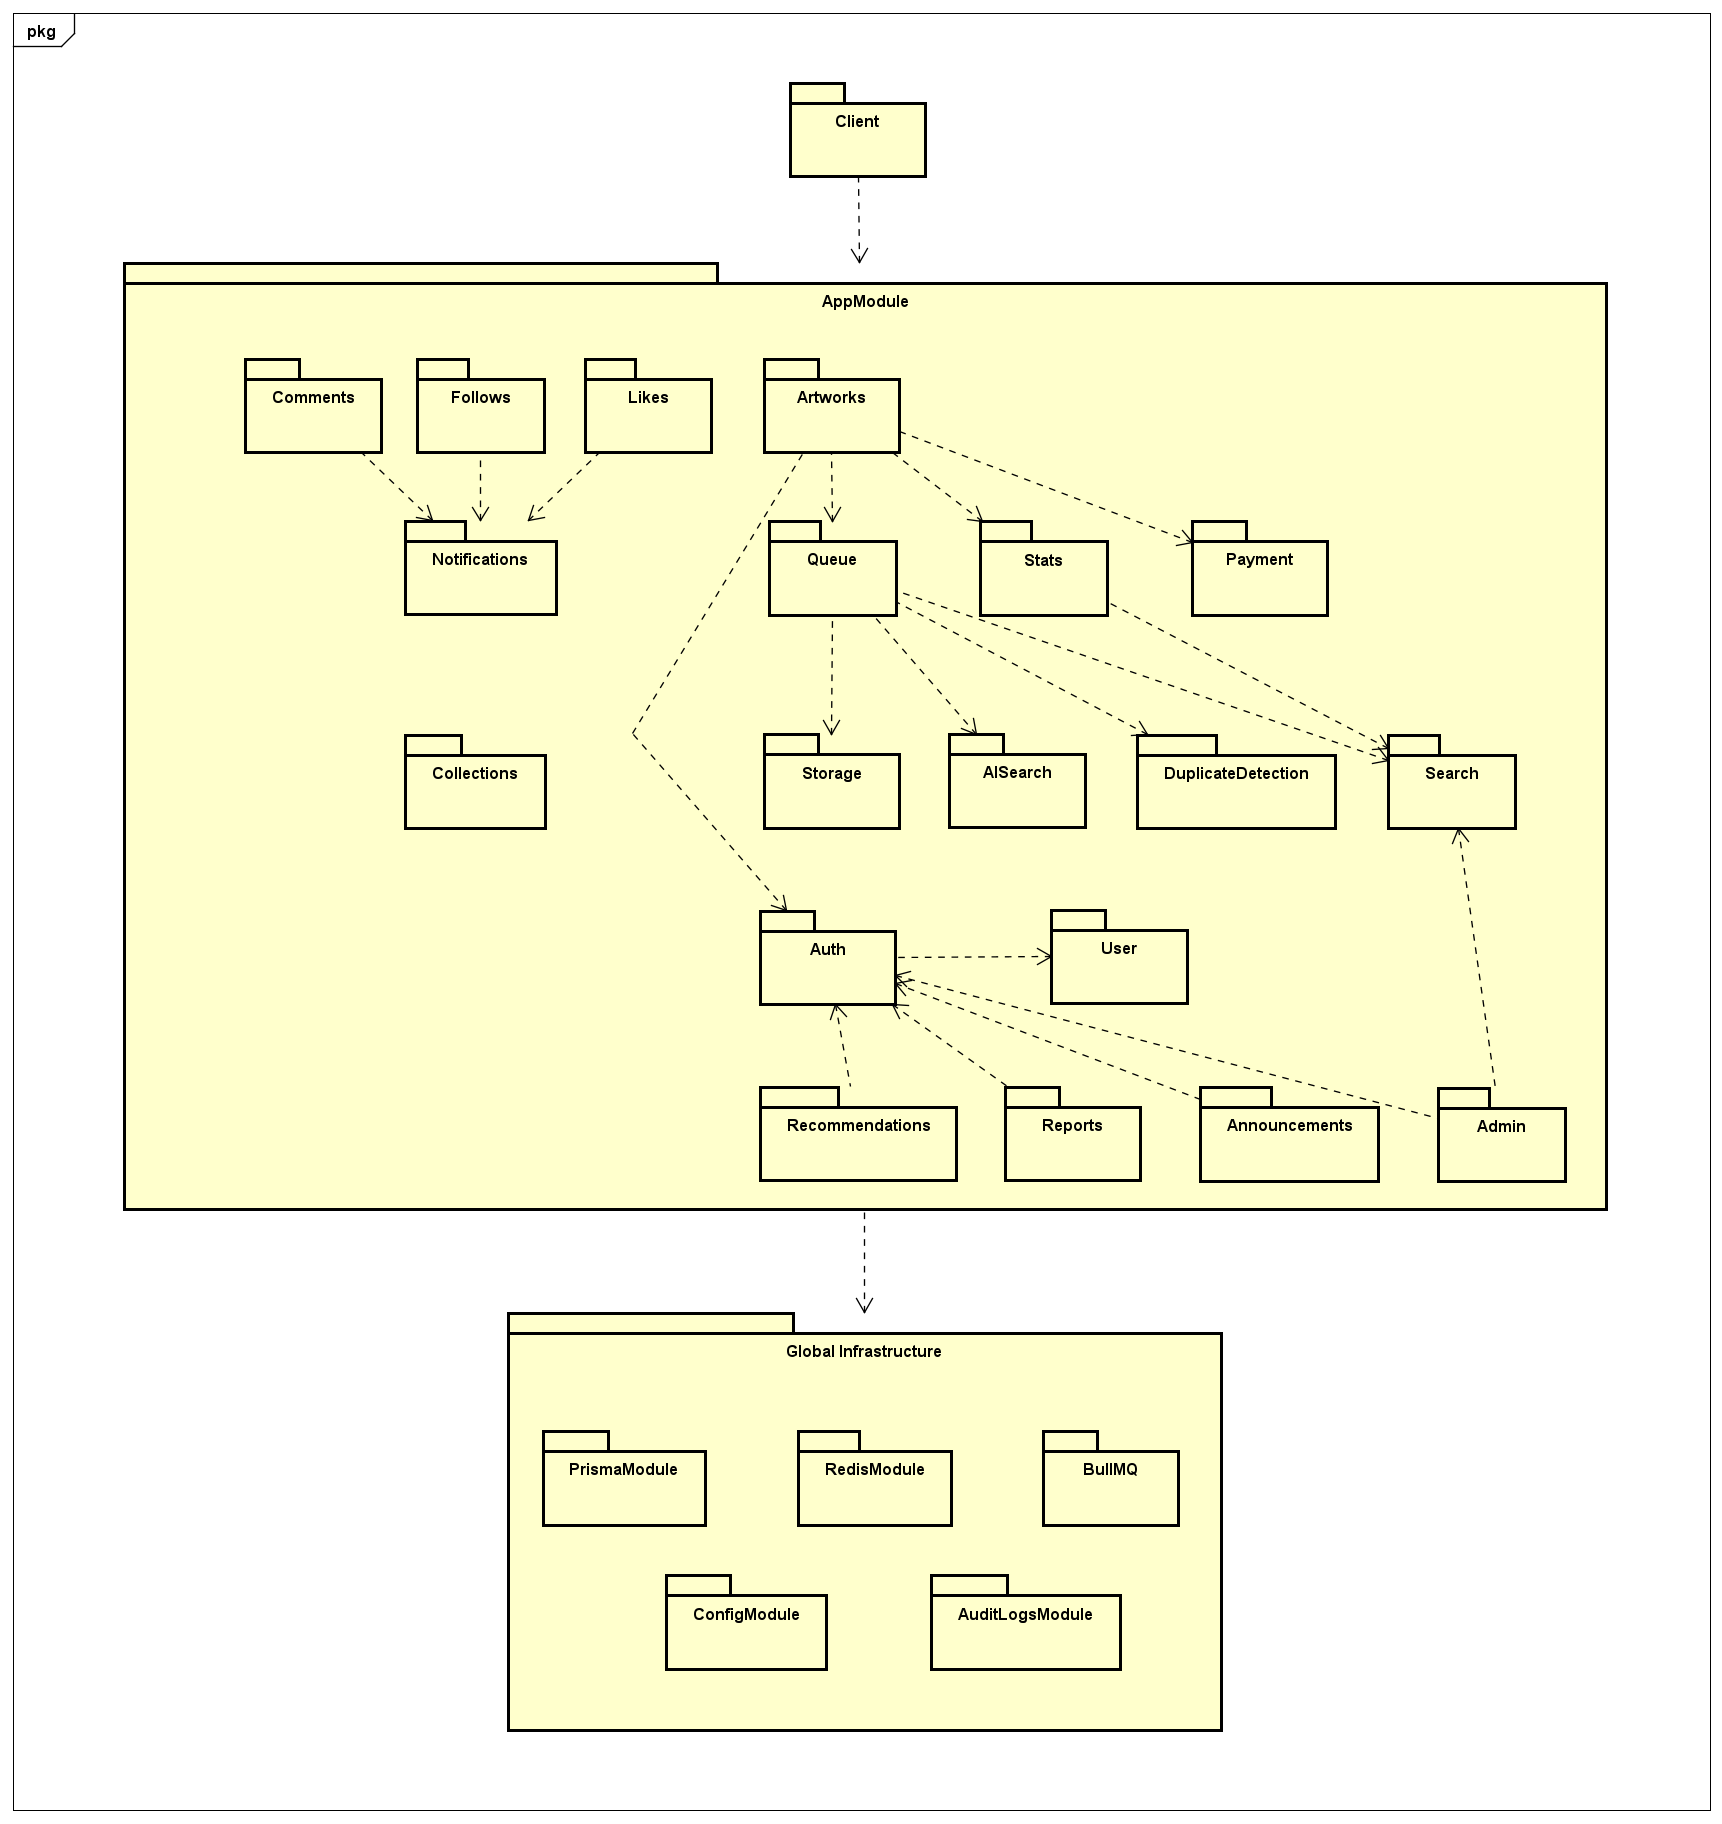
\includegraphics[width=0.85\linewidth]{Hinh_4_1_Bieu_do_phu_thuoc_goi.png}
\caption{Biểu đồ phụ thuộc mô-đun tổng quan của hệ thống}
\label{fig:4_1}
\end{figure}

Các mô-đun được nhóm thành các cụm nghiệp vụ logic như sau:

1. Cụm Nội dung cốt lõi: Bao gồm mô-đun Artworks (quản lý tác phẩm nghệ thuật, là trung tâm của hệ thống với số lượng phụ thuộc lớn nhất) và mô-đun Collections (bộ sưu tập cá nhân).

2. Cụm Danh tính và Truy cập: Bao gồm mô-đun Auth (xác thực qua Clerk) và mô-đun Users (quản lý hồ sơ). Đây là cặp mô-đun duy nhất trong hệ thống tồn tại phụ thuộc vòng hai chiều (circular dependency), được xử lý thông qua cơ chế forwardRef của NestJS.

3. Cụm Tương tác xã hội: Bao gồm mô-đun Likes, Comments và Follows. Cả ba đều phụ thuộc vào mô-đun Notifications để gửi thông báo thời gian thực khi có tương tác mới.

4. Cụm Thanh toán: Mô-đun Payments tích hợp trực tiếp với Stripe \cite{stripe} để quản lý vòng đời gói hội viên định kỳ (subscription).

5. Cụm Xử lý và Thông minh: Bao gồm mô-đun Queue (đường ống xử lý ảnh nền), Stats (thống kê lượt xem), Search (tìm kiếm toàn văn qua Meilisearch), AiSearch (tìm kiếm ngữ nghĩa qua Gemini và pgvector), DuplicateDetection (phát hiện ảnh trùng lặp qua pHash), và Recommendations (gợi ý cá nhân hóa). Mô-đun Queue đóng vai trò trung tâm xử lý, kết nối với Storage, Search, DuplicateDetection và AiSearch để thực hiện đường ống xử lý ảnh hoàn chỉnh sau khi người dùng tải lên.

6. Cụm Quản trị: Bao gồm mô-đun Admin (bảng điều khiển quản trị), Reports (báo cáo vi phạm), và Announcements (thông báo hệ thống). Cả ba đều phụ thuộc vào Auth để xác thực quyền quản trị viên.

7. Hạ tầng toàn cục: Nằm ở dưới cùng biểu đồ, bao gồm PrismaModule (kết nối PostgreSQL \cite{postgresql}), RedisModule (bộ nhớ đệm), BullMQ (hàng đợi tin nhắn) \cite{bullmq}, ConfigModule (cấu hình môi trường), và AuditLogsModule (ghi nhật ký kiểm toán). Tất cả mô-đun nghiệp vụ đều ngầm phụ thuộc vào tầng này.

\subsection{Thiết kế chi tiết gói}
\label{subsection:4.1.3}

Sau khi xác định kiến trúc tổng thể, do hệ thống có hơn 25 mô-đun phức tạp đan xen nhau, phần này áp dụng nguyên lý thiết kế hướng miền (Domain-Driven Design - DDD) để phân tách hệ thống thành 5 cụm (nhóm package) có liên quan mật thiết về mặt nghiệp vụ. Việc bóc tách này giúp làm rõ các ranh giới dịch vụ và chức năng trong kiến trúc Modular Monolith. Mỗi biểu đồ thiết kế gói dưới đây sẽ trình bày các lớp (class) và mối quan hệ giữa chúng trong nội bộ nhóm.

\textbf{1. Nhóm Định danh và Quản lý Người dùng (Identity \& Access)}

Nhóm này bao gồm AuthModule và UsersModule, đóng vai trò cửa ngõ kiểm soát quyền truy cập và lưu trữ hồ sơ thành viên của toàn hệ thống. Hình 4.2 minh họa thiết kế chi tiết của nhóm.

\begin{figure}[H]
\centering
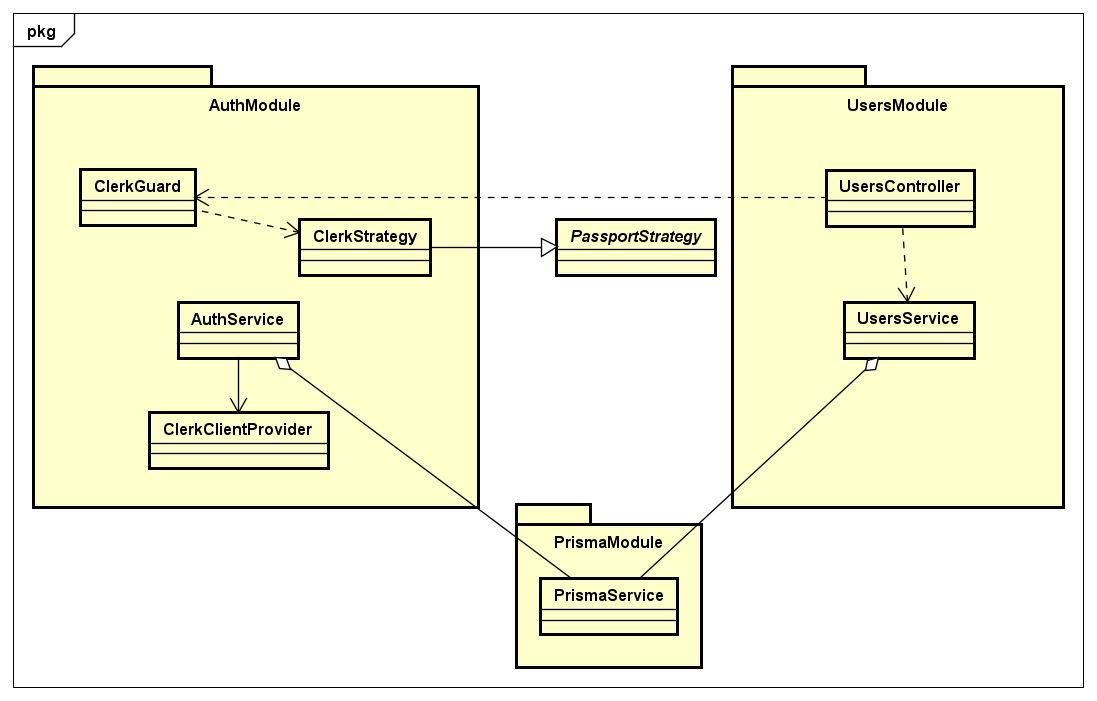
\includegraphics[width=0.85\linewidth]{Hinh_4_2_Thiet_ke_goi_Identity.png}
\caption{Thiết kế chi tiết nhóm Định danh và Quản lý Người dùng}
\label{fig:4_2}
\end{figure}

Bên trong AuthModule, lớp ClerkStrategy có quan hệ kế thừa (inheritance) từ lớp trừu tượng PassportStrategy, triển khai chiến lược xác thực dựa trên JWT từ Clerk \cite{clerk}. ClerkGuard phụ thuộc vào AuthService để kích hoạt luồng xác thực. Điểm đáng chú ý là AuthService phụ thuộc UsersService để tra cứu người dùng nội bộ, trong khi UsersService phụ thuộc AuthService để xác minh danh tính, tạo thành quan hệ phụ thuộc vòng (circular dependency) được giải quyết bằng forwardRef. Tuy nhiên, cả hai lớp Service đều duy trì quan hệ kết tập (aggregation) với PrismaService để giao tiếp độc lập với cơ sở dữ liệu.

\textbf{2. Nhóm Lõi Nội dung và Xử lý Ảnh (Core Content \& Processing)}

Đây là "trái tim" của hệ thống, xử lý luồng tải lên và phân phối nội dung, bao gồm ArtworksModule, CollectionsModule, StorageModule và QueueModule. Hình 4.3 minh họa thiết kế.

\begin{figure}[H]
\centering
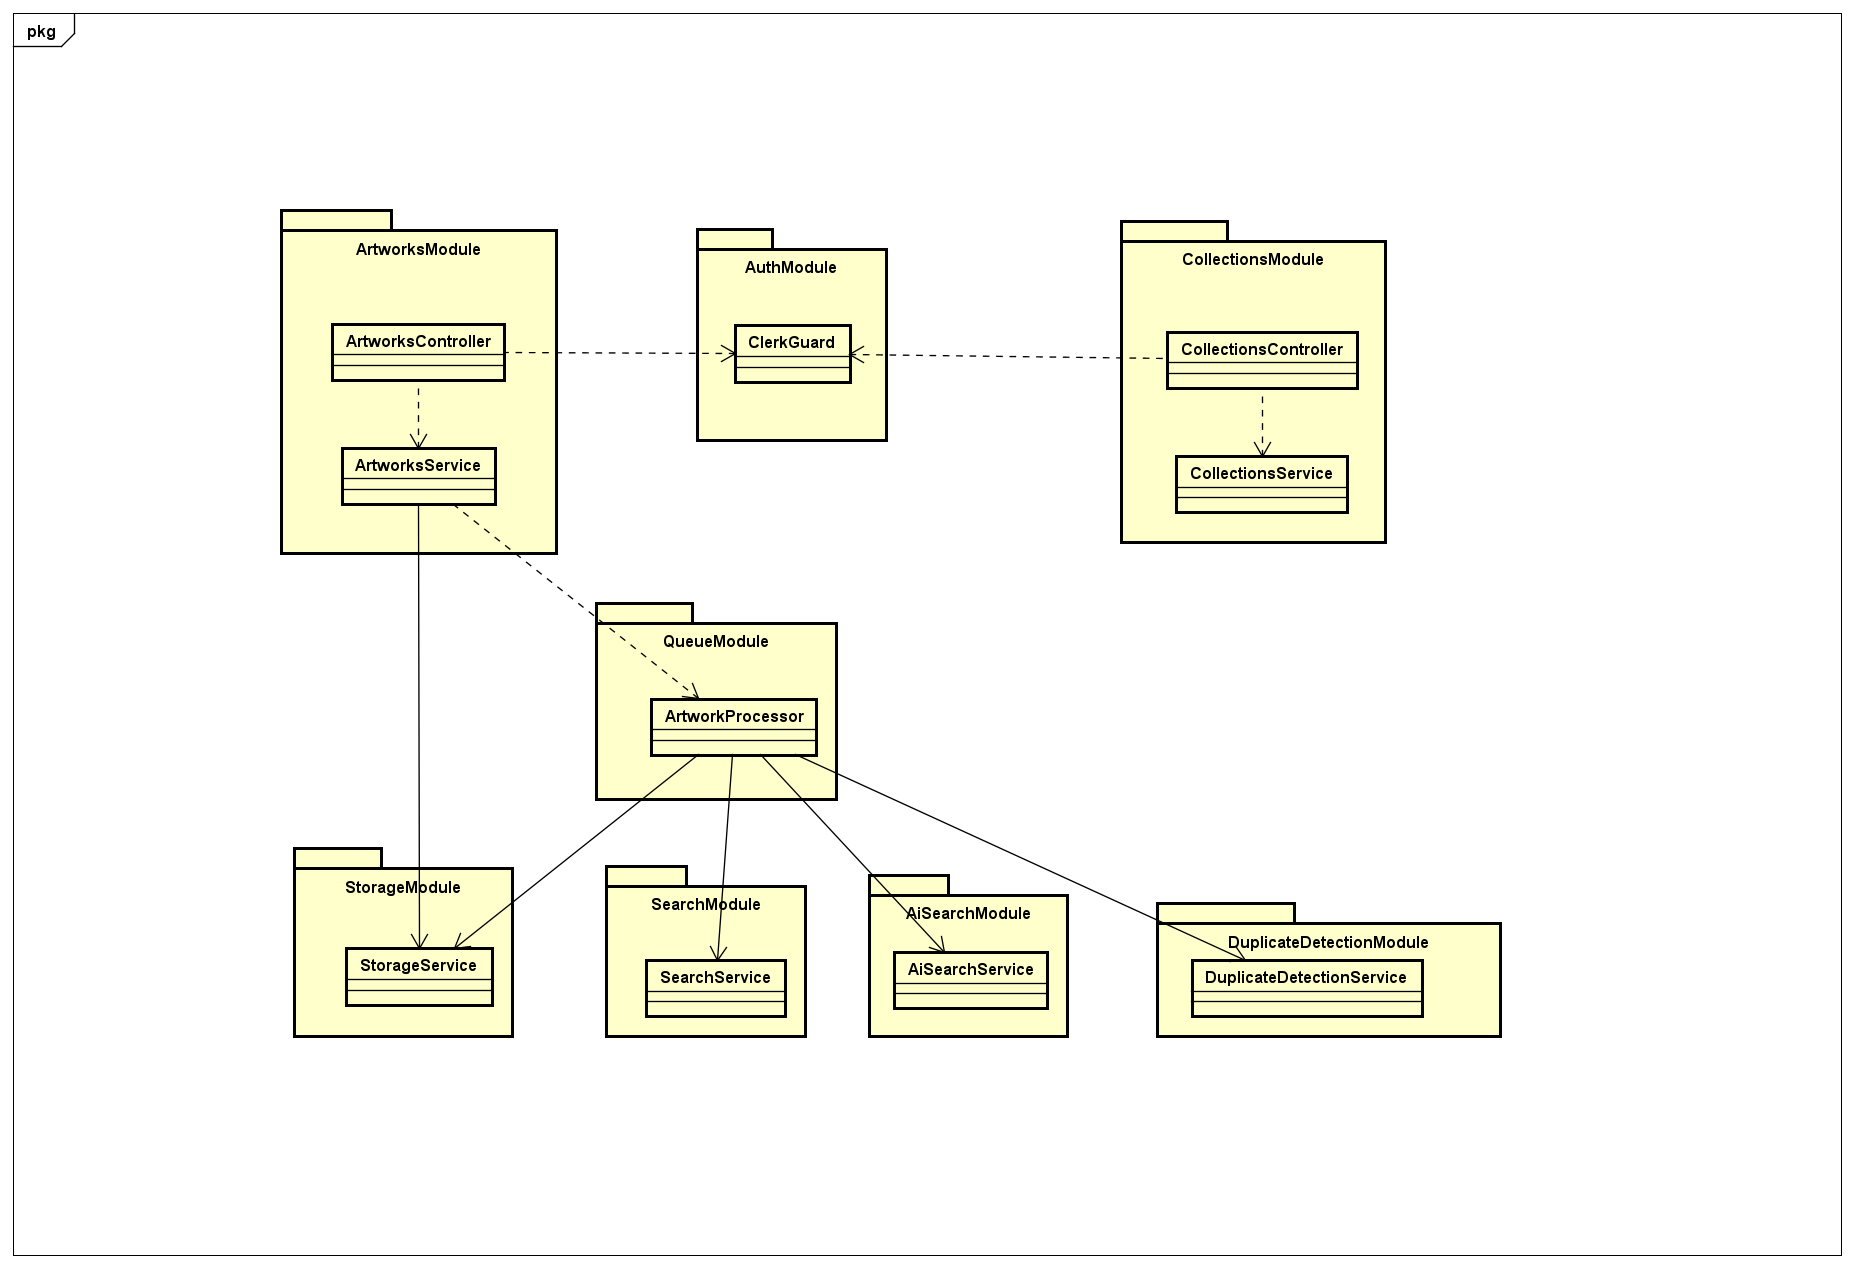
\includegraphics[width=0.85\linewidth]{Hinh_4_3_Thiet_ke_goi_Core.png}
\caption{Thiết kế chi tiết nhóm Lõi Nội dung và Xử lý Ảnh}
\label{fig:4_3}
\end{figure}

ArtworksController và CollectionsController đều phụ thuộc vào ClerkGuard để bảo vệ các API. Lớp ArtworksService gọi đến lớp ArtworkProcessor (thuộc QueueModule) để khởi tạo quy trình xử lý nền không đồng bộ, giúp luồng chính của máy chủ không bị nghẽn (non-blocking). Từ ArtworkProcessor, các luồng dữ liệu được đẩy thẳng sang StorageService để lưu ảnh vào MinIO, cũng như đẩy đến các dịch vụ AI và tìm kiếm bên ngoài mà không làm ảnh hưởng đến thời gian phản hồi của ArtworksModule. 

\textbf{3. Nhóm Tương tác Xã hội \& Cảnh báo (Social Interactions \& Notifications)}

Nhóm này quản lý các hoạt động cộng đồng, bóc tách hoàn toàn logic tương tác khỏi phần lõi nội dung, bao gồm LikesModule, CommentsModule, FollowsModule và NotificationsModule. Hình 4.4 minh họa thiết kế.

\begin{figure}[H]
\centering
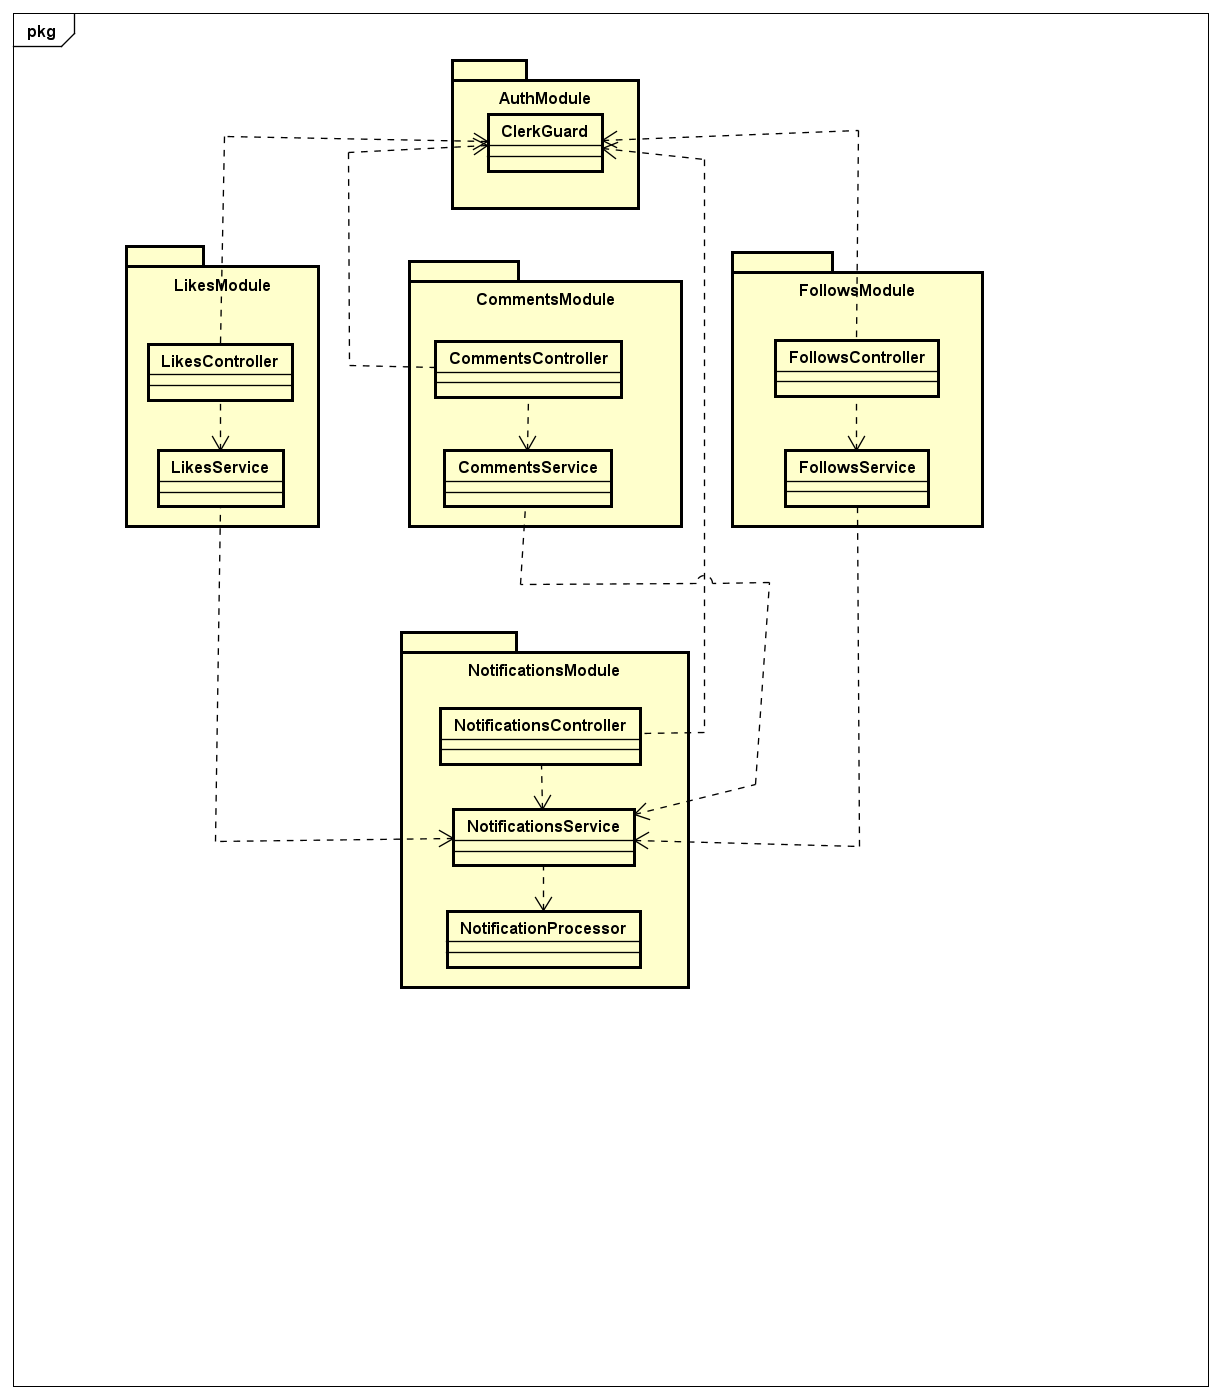
\includegraphics[width=0.85\linewidth]{Hinh_4_4_Thiet_ke_goi_Social.png}
\caption{Thiết kế chi tiết nhóm Tương tác Xã hội và Cảnh báo}
\label{fig:4_4}
\end{figure}

Đặc điểm kiến trúc nổi bật nhất của nhóm này là LikesService, CommentsService và FollowsService đều có quan hệ phụ thuộc (dependency) một chiều trỏ về NotificationsService. Thiết kế này tuân thủ chặt chẽ nguyên tắc Loose Coupling, cho phép các hành động tương tác (như thả tim, bình luận) dễ dàng kích hoạt thông báo theo thời gian thực (real-time) tới người dùng nhận mà không làm phình to logic nội bộ của bản thân chức năng tương tác đó.

\textbf{4. Nhóm Xử lý Dữ liệu Thông minh (Intelligence \& Search)}

Nhóm này tập trung vào bài toán khám phá nội dung bằng văn bản và trí tuệ nhân tạo, bao gồm SearchModule, AiSearchModule, DuplicateDetectionModule, RecommendationsModule và StatsModule. Hình 4.5 minh họa thiết kế.

\begin{figure}[H]
\centering
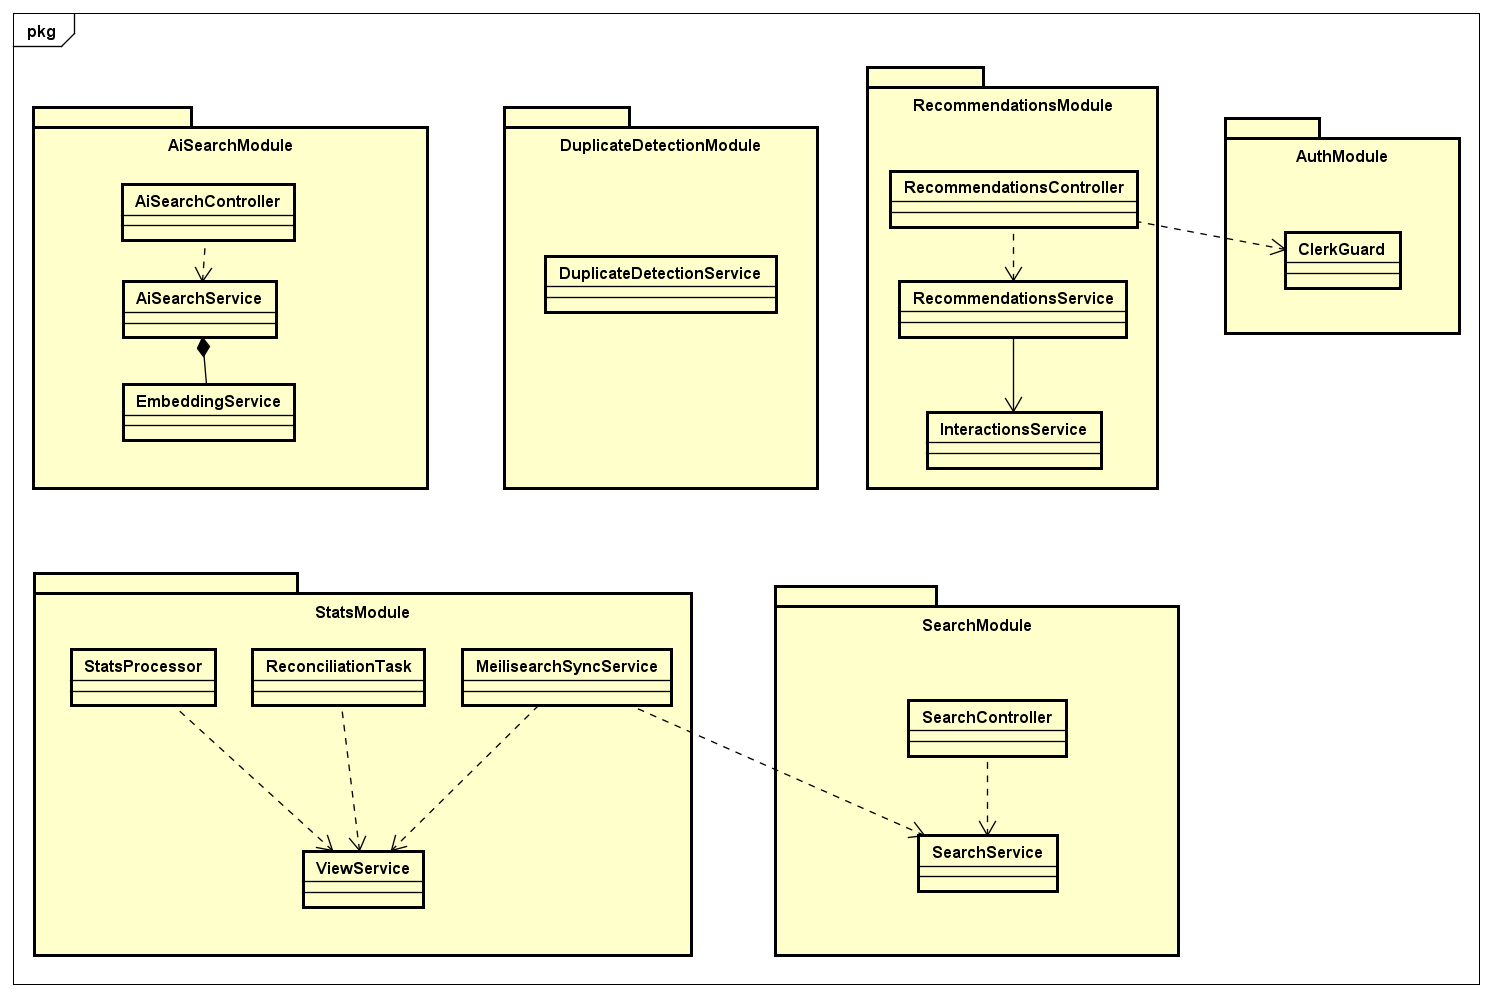
\includegraphics[width=0.85\linewidth]{Hinh_4_5_Thiet_ke_goi_Intelligence.png}
\caption{Thiết kế chi tiết nhóm Xử lý Dữ liệu Thông minh}
\label{fig:4_5}
\end{figure}

Bên trong AiSearchModule, lớp EmbeddingService có quan hệ hợp thành (composition) với AiSearchService, tạo thành một cụm chuyên biệt gọi API Gemini để trích xuất vector ngữ nghĩa hình ảnh. MeilisearchSyncService (thuộc StatsModule) phụ thuộc trực tiếp vào SearchService để đồng bộ dữ liệu tìm kiếm siêu tốc độ. Đặc biệt, RecommendationsModule được thiết kế theo kiến trúc Hướng sự kiện (Event-Driven) để thu thập hành vi người dùng (như lượt xem, lượt thích) thông qua InteractionsService. Thay vì bắt các module chức năng gọi chéo lẫn nhau, hệ thống sử dụng Event Emitter để duy trì tính độc lập lỏng lẻo (Loose Coupling) tuyệt đối. Đây là cụm module tập hợp các công nghệ phức tạp nhất như pgvector và mã băm pHash để cung cấp trải nghiệm tìm kiếm ảnh chính xác và gợi ý cá nhân hóa.

\textbf{5. Nhóm Quản trị, Vận hành và Doanh thu (Management \& Monetization)}

Nhóm này chịu trách nhiệm quản lý hệ thống Backoffice (dành cho Admin) và xử lý luồng doanh thu, hoàn toàn tách biệt khỏi trải nghiệm lướt web thông thường của người dùng cuối. Nhóm bao gồm AdminModule, ReportsModule, AnnouncementsModule, PaymentsModule và AuditLogsModule. Hình 4.6 minh họa thiết kế.

\begin{figure}[H]
\centering
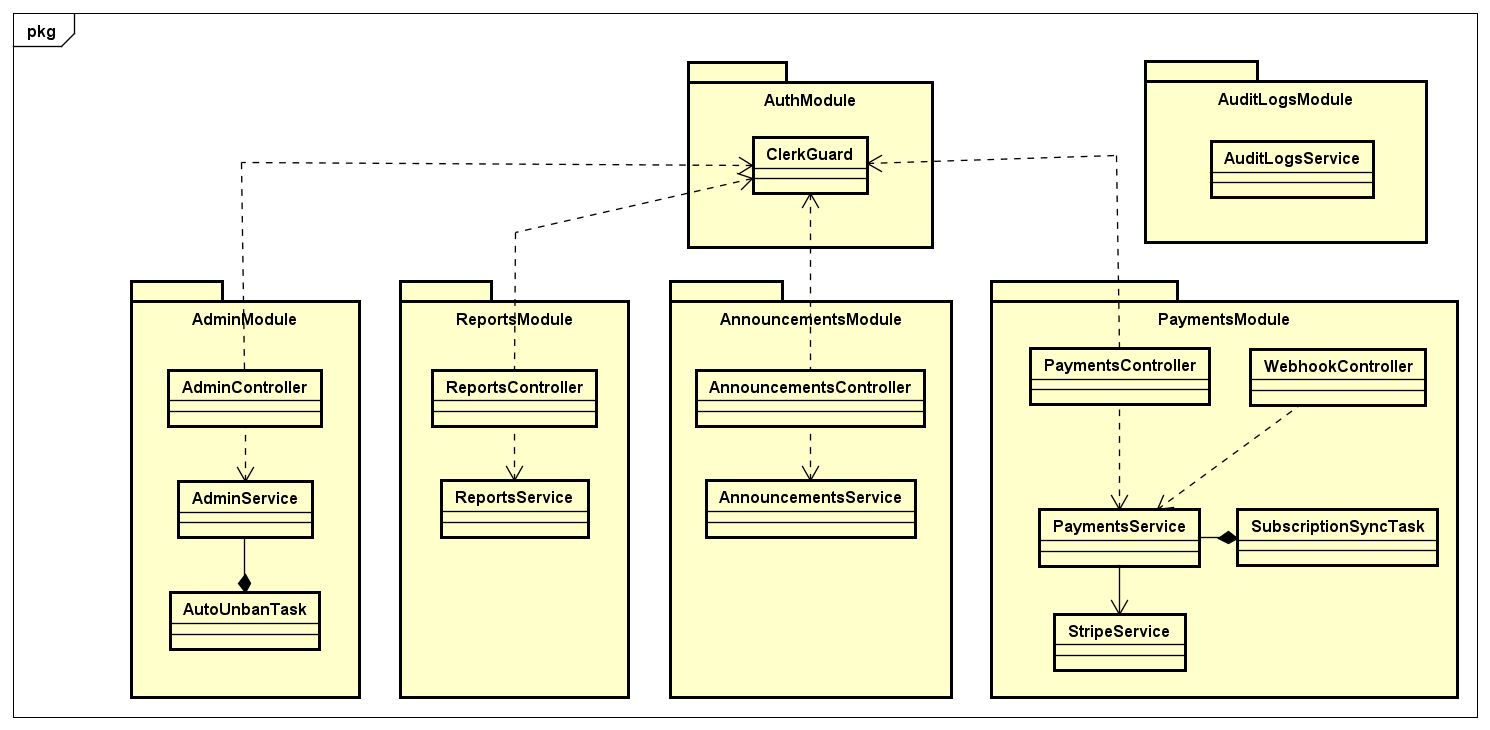
\includegraphics[width=0.85\linewidth]{Hinh_4_6_Thiet_ke_goi_Management.png}
\caption{Thiết kế chi tiết nhóm Quản trị, Vận hành và Doanh thu}
\label{fig:4_6}
\end{figure}

PaymentsModule cung cấp PaymentsController cho người dùng trích xuất hóa đơn và WebhookController để lắng nghe sự kiện từ cổng thanh toán Stripe. Điểm chung của cụm nghiệp vụ này là sử dụng nhiều tác vụ chạy ngầm (CronJob) có quan hệ hợp thành với Service nội bộ, điển hình như AutoUnbanTask thuộc AdminService (để tự động mở khóa tài khoản) và SubscriptionSyncTask thuộc PaymentsService (để đồng bộ gói hội viên).

Cuối cùng, Hình 4.7 (sẽ được đính kèm ở bản vẽ khổ lớn đính kèm cùng báo cáo) trình bày bức tranh tổng thể mạng lưới chi tiết nhất về toàn bộ cấu trúc lớp và mối liên kết phức tạp giữa toàn bộ hơn 25 mô-đun trong hệ thống Modular Monolith của nền tảng.


\section{Thiết kế cơ sở dữ liệu}
\subsection{Mô hình thực thể quan hệ}
\subsection{Thiết kế bảng người dùng và phân quyền}
\subsection{Thiết kế bảng tác phẩm và ảnh}
\subsection{Thiết kế bảng tương tác xã hội}
\subsection{Thiết kế bảng thanh toán và gói thành viên}

\section{Thiết kế API và giao tiếp hệ thống}
\subsection{API xác thực và người dùng}
\subsection{API quản lý tác phẩm}
\subsection{API tìm kiếm và khám phá}
\subsection{API quản trị và kiểm duyệt}
\subsection{API thanh toán và webhook}

\section{Triển khai hệ thống}
\subsection{Môi trường phát triển}
\subsection{Cấu hình cơ sở dữ liệu và dịch vụ trung gian}
\subsection{Triển khai frontend}
\subsection{Triển khai backend}
\subsection{Triển khai worker xử lý nền}

\section{Đánh giá và kiểm thử}
\subsection{Kiểm thử chức năng}
\subsection{Kiểm thử tích hợp}
\subsection{Đánh giá hiệu năng xử lý ảnh}
\subsection{Đánh giá tìm kiếm}
\subsection{Đánh giá bảo mật và phân quyền}


\chapter{CÁC GIẢI PHÁP VÀ ĐÓNG GÓP NỔI BẬT}
\label{chapter:contributions}
\section{Tự động hóa pipeline xử lý ảnh}
\subsection{Tách tác vụ nặng khỏi luồng request}
\subsection{Quản lý tiến độ và trạng thái xử lý}
\subsection{Xử lý lỗi cục bộ ở cấp ảnh}

\section{Kiểm duyệt nội dung bán tự động}
\subsection{Phân loại NSFW trong worker}
\subsection{Lưu metadata phục vụ điều phối}
\subsection{Cân bằng giữa tự động hóa và kiểm duyệt thủ công}

\section{Phát hiện ảnh trùng lặp bằng pHash}
\subsection{Sinh dấu vân tay nhận thức}
\subsection{So sánh bằng khoảng cách Hamming}
\subsection{Ứng dụng trong bảo vệ nội dung}

\section{Tìm kiếm lai toàn văn và ngữ nghĩa}
\subsection{Lập chỉ mục Meilisearch}
\subsection{Lưu trữ vector bằng pgvector}
\subsection{Kết hợp kết quả tìm kiếm trong trải nghiệm người dùng}

\section{Mô hình thành viên cho người sáng tạo}
\subsection{Thiết kế artist tier}
\subsection{Tích hợp Stripe subscription}
\subsection{Kiểm soát quyền truy cập nội dung}


\chapter{KẾT LUẬN VÀ HƯỚNG PHÁT TRIỂN}
\label{chapter:conclusion}
\section{Kết luận}
\subsection{Kết quả đạt được}
\subsection{Mức độ đáp ứng mục tiêu đề tài}
\subsection{Các hạn chế còn tồn tại}

\section{Hướng phát triển}
\subsection{Mở rộng khả năng kiểm duyệt}
\subsection{Tối ưu tìm kiếm vector}
\subsection{Cải tiến hệ thống khuyến nghị}
\subsection{Mở rộng cơ chế bản quyền và khiếu nại}
\subsection{Tối ưu triển khai hạ tầng quy mô lớn}


\newpage
\renewcommand\bibname{TÀI LIỆU THAM KHẢO}
\printbibliography
\addcontentsline{toc}{chapter}{TÀI LIỆU THAM KHẢO}

\end{document}
